% !TEX root = free234.tex
\chapter{Vector Calculus}
\section{Vector Fields}
So far we have been studying the calculus of \textit{functions} of several
variables.  Functions are used to describe things that have different values at
different locations, e.g.~quantities like temperature, or density.  Many other
physical phenomena are described by \emph{vector fields,} i.e.~by vectors whose
direction and magnitude can vary from place to place.  Vector calculus is the
theory of integration and differentiation of vector fields.

By definition, a vector field in the plane is a vector valued function of two
variables: whereas
an ordinary function of two variables gives us a number for each $(x, y)$ in its
domain, a vector field gives us a vector in the plane for each point $(x,y)$ in
its domain.  Such a vector is determined by its two components, both of which
are ordinary functions of $(x, y)$.  The notation we will use in this course is
as follows:
\begin{equation}
  \vv(x, y) = \vek P(x, y) \\ Q(x, y)\tor = 
  P(x,y) \vi + Q(x, y) \vj.
  \label{eq:05vectorfield-notation}
\end{equation}

For a vector field in three dimensional space we must specify a vector $\vv(x,
y, z)$ at each point $(x, y, z)$ in a three dimensional domain :
\[
\vv(x, y) = \vek P(x, y) \\ Q(x, y) \\ R(x, y)\tor = P(x,y) \vi + Q(x, y) \vj +
R(x, y)\vk.
\]
To draw a vector field in the plane we would have compute $\vv(x, y)$ at lots of
points and simply plot them.  The more points we pick, the busier the picture
gets.  See for example Figure~\ref{fig:05grad-theta}, in which the vector field
\begin{equation}\label{eq:05grad-theta}
  \vv(x, y) = \vek -y / (x^2+y^2)\\ x/(x^2+y^2) \tor
\end{equation}
is drawn.


\section{Examples of vector fields}
\label{sec:vector-field-examples}
\subsection{Gradients as vector fields}
\label{sec:gradient-is-vector-field}
We have already seen examples of vector fields before, namely
{\itshape the gradient of any function $f(x, y)$ is a vector field:}
\[
\nab f(x, y) = \vek f_x(x, y) \\ f_y(x, y)\tor.
\]
In fact, the example (\ref{eq:05grad-theta}) is such a vector field: it is the
gradient of the polar angle $\theta$.  In \S III.\ref{sec:functions-in-PC-theta}
we saw that for $x>0$ this angle is given by $\theta(x, y)$, and we checked in
problem~III.\ref{prb:grad-of-theta} that $\vv$ given by (\ref{eq:05grad-theta}) and
shown below in Figure~\ref{fig:05grad-theta} satisfies $\vv = \nab \theta$.
\begin{figure}[t]
  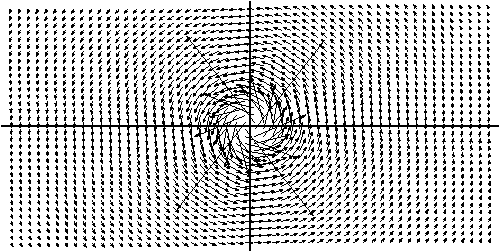
\includegraphics[scale=1]{05vectorfield.pdf}
  \caption{\textbf{A vector field in the plane.}  This vector field is\\[1ex]
    \null\qquad$\DS
    \vv(x, y) = \nab \theta(x, y) = \frac{-y}{x^2+y^2}\vi + \frac{x}{x^2+y^2}\vj$.
    \\[1ex]
    In general, drawings of vector fields become messy in the region where the
    vectors are long, because they tend to overlap.  Drawing a three dimensional
    vector field is challenging.}
  \label{fig:05grad-theta}
\end{figure}

\subsection{Fluid flow}\label{sec:fluid-flow}   
Vector fields appear in various ways in physics.  The easiest way to visualize a
vector field is by thinking of it as the velocity field of a fluid flow.  Suppose a
fluid is flowing through a certain region in space.  The velocities of the fluid
particles will generally vary from place to place, and also with time.  A fluid flow
is called \textit{steady} if the velocity of a fluid particle only depends on its
location.  This means that the velocity vector $\vv$ of a fluid particle is a
function of its coordinates $(x, y, z)$ only, and does not depend on time.

\begin{figure}[ht]
  \centering
  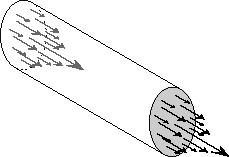
\includegraphics{05poiseuille3D.pdf}\qquad
  \begin{picture} (200.000000,105.125000)(0,0)
    \put(0.0, 0.0){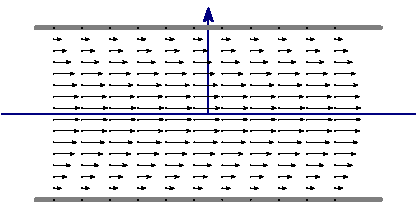
\includegraphics{05poiseuille.pdf}}
        \put(182.50,  52.50){\sffamily\itshape central axis}
    \put(104.00,  95.88){\sffamily\itshape $r$}
    \put(184.50,  89.88){\sffamily\itshape wall}

\end{picture}

  \caption{\textbf{Fluid flow in a cylindrical pipe.  } \textbf{Left: } as a viscous
  fluid flows through a pipe it sticks to the walls, and so its velocity will be
  highest at the center of the pipe.  \textbf{Right: } a drawing of a cross section
  the flow on the left.  We see the vector field corresponding to so-called
  \textit{Poiseuille flow,} given by Equation~(\ref{eq:05poisseuille-flow}).  }
  \label{fig:05poisseuille-flow}
\end{figure}

For instance, if a viscous fluid flows through a cylindrical pipe, the velocity of
the fluid will only depend on the distance to the central axis of the pipe.  On the
walls the velocity will vanish (the fluid sticks to the wall of the pipe), and in the
center the fluid will move fastest.  Under certain circumstances it follows from the
laws of fluid mechanics that the velocity field
\begin{itemize}
\item is always parallel to the central axis, and

\item depends quadratically on the distance to the central axis.

\end{itemize}
It is given by
\begin{equation}
  \label{eq:05poisseuille-flow}
  \vv(x, y, z) = v_c\, \bigl(1-\frac{r^2} {R^2}\bigr)\vi
  = \vek v_c \bigl(1-(r/R)^2\bigr) \\ 0\\0\tor ,
\end{equation}
where $R$ is the radius of the pipe, $r$ is the distance to its central axis,
and $v_c$ is the velocity at the center of the pipe.

This example describes the motion of a fluid, but a vector field can be the
velocity field of anything that moves, in particular, a gas flow has a velocity
field, and the velocities in a moving elastic solid (think ``Jello'') must also
be described by a vector field.

\subsection{Force fields}    
\label{sec:force-field-examples}
If we assume the Earth is flat, then the gravitational force it exerts on a mass
$m$ is always the vector $\vF = \tvek 0 \\ -mg\ttor$.  We can think of this as a
constant vector field: its magnitude and direction are the same everywhere.

But the Earth is not flat, and according to Newton the gravitational force $\vF$
is a vector pointing towards the center of the earth, whose magnitude is
inversely proportional to the distance to the center of the Earth.  If we choose
the Earth's center to be the origin, then Newton's law looks like this:
\begin{equation}
  \label{eq:05Newton-on-gravity}
  \vF(x, y, z) = -C \frac{\vx}{\|\vx\|^3}, \qquad \vx = \vek x\\y\\z\tor.
\end{equation}
\marginpar{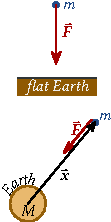
\includegraphics[scale=1.25]{05newtons-law.pdf}}%
Here $C$ is a constant that depends on the mass $m$ of the object, and the mass $M$ of
the Earth (physics tells us that $C= GMm$, where $G$ is called the ``universal gravitational constant.'')

Other prominent examples of vector fields appear in the theory of
electromagnetism.  The electric currents and charges around us create an
electric field and a magnetic field, which at each point in space are given by
vectors $\vE$ and $\vB$.  These vectors change from place to place, and so they
define vector fields
\[
\vE = \vE(x, y, z), \qquad \vB=\vB(x, y, z).
\]
For example, Coulomb's law states that the electric field generated by a charged
particle at the origin is given by
\begin{equation}
  \label{eq:05coulombs-law}
  \vE(x, y, z) = \frac{Q} {4\pi\epsilon_0} \frac{\vx} {\|\vx\|^3},
\end{equation}
which is almost the same as Newton's law (\ref{eq:05Newton-on-gravity}) for the
gravitational field.  Here $\epsilon_0$ is some constant, and $Q$ is the
electric charge of the particle.

If an electric current of strength $I$ runs upward through the $z$-axis, then
this current will create a magnetic field which is given by
\begin{equation}
  \label{eq:05field-of-current}
  \vB(x, y, z) = \frac{\mu_0 I} {2\pi}
  \vek -y/(x^2+y^2) \\ x/(x^2+y^2) \\ 0 \tor.
\end{equation}
Again, a constant ($\mu_0$) appears.  If we compare
(\ref{eq:05field-of-current}) with (\ref{eq:05grad-theta}), then we see that,
except for the constant factor $\mu_0 I /2\pi$ this vector field is a three
dimensional version of the one drawn in Figure~\ref{fig:05grad-theta}: we can
regard Figure~\ref{fig:05grad-theta} as a ``top view'' of the magnetic field
$\vB$ of an electric
current. \marginpar{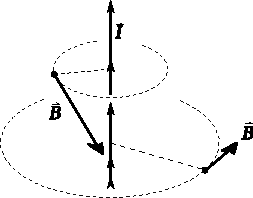
\includegraphics[scale=0.8]{05magneticfield.pdf}}

\section{Line integrals}

\subsection{Line integrals of functions}
\label{sec:line-integral-of-function}%
Instead of integrating over plane domains, or regions in space, it often turns
out to be useful to integrate over a curve in the plane, or a curve in space.

If $\cC$ is a curve in the plane, or in space, (think of a line segment, a
circular arc, or a fancier curve), and if $w=f(x, y, z)$ is a function then the
basic pattern for defining the integral of $f$ over the curve $\cC$ is the same
as for all the other integrals we have defined in the previous chapter.

\begin{figure}[h]
  \begin{picture} (120.000000,70.833333)(0,0)
    \put(0.0, 0.0){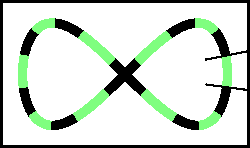
\includegraphics{05curve-partitioned.pdf}}
        \put(113.15,  34.83){\sffamily\itshape $\updownarrow\Delta s$}

\end{picture}

  \caption{Partitioning a curve.}
  \label{fig:05partitioning-a-curve}
\end{figure}
To define the integral we divide the curve $\cC$ into many short arcs, and label
them $\cC_1$, \ldots, $\cC_n$; we choose one sample point $(x_k, y_k, z_k)$ on
arc $\cC_k$ for every $k=1, \cdots, n$; and we compute the length $\Delta s_k$
of each arc $\cC_k$.  With these data we form the Riemann sum
\begin{equation}
  \cR = f(x_1, y_1, z_1)\Delta s_1 + \cdots 
  + f(x_n, y_n, z_n)\Delta s_n,
  \label{eq:05line-integral-riemann-sum}
\end{equation}
and if these Riemann sums converge as one makes the partition arbitrarily fine,
then we call the limit the line integral of $f$ with respect to arc length over
the curve $\cC$:
\begin{equation}
  \int_\cC f(x, y, z) \; ds
  = 
  \lim_{%
    \parbox{6em}
    {\footnotesize\sffamily
      \centering{``as the partition\\ gets finer''}}
  }  \sum _{k=1}^n f(x_k, y_k, z_k)\Delta s_k.
  \label{eq:05line-integral-defined}
\end{equation}
The length of the curve $\cC$ can be expressed as a line integral
\[
\text{Length of }\cC = \int_\cC\; ds.
\]

\begin{figure}[t]
  \input ../figures/234/05curve-and-tangent.pdf_tex
  \caption{\textbf{A parametrized curve: } \textbf{Left: } The vector $\vx'(t)$
    is tangent to the curve at the point $\vx(t)$.  The vector $\vx(t)$ is the
    position vector of a point on the curve.  \textbf{Right: } Increasing the
    parameter $t$ by a small amount $\Delta t$ changes the position vector to
    $\vx(t+\Delta t)$, causing the corresponding point on the curve to move by
    $\vx(t+\Delta t) - \vx(t) \approx \vx'(t) \Delta t$.  }
\end{figure}
\subsection{How to calculate a line integral}
\label{sec:how-to-compute-int-fds}%
Recall that a curve $\cC$ is usually given by a parametrization
\[
\vx=\vx(t)=\vek x(t)\\y(t)\\z(t)\tor,\; (a\leq t\leq b)
\]
also written as $\vx(t) = x(t)\vi + y(t) \vj + z(t) \vk$.

Given such a parametrization it is easy to make partitions by just partitioning
the parameter interval $a\leq t\leq b$ into many short sub intervals, $a=t_0 <
t_1 < \cdots < t_n =b$.  We could choose the $k^{\rm th}$ sample point to be the
point $\vx(t_k)$.  The length of the arc from $\vx(t_{k-1})$ to $\vx(t_k)$ is
approximately the same as the distance between these two points (for as one
makes the partition finer, the arcs become more and more like short line
segments).  Thus we find
\[
\Delta s_k \approx \|\vx(t_{k}) - \vx(t_{k-1})\| =\left\| \frac{\vx(t_{k}) -
    \vx(t_{k-1})}{\Delta t_k} \right\|\; \Delta t_k \approx \|\vx'(t_k)\| \;
\Delta t_k,
\]
where $\Delta t_k = t_k-t_{k-1}$.  The Riemann sum for the line integral is
\[
\cR \approx \sum_{k=1}^n f(\vx(t_k)) \; \|\vx'(t_k)\|\; \Delta t_k.
\]
As the partition is made finer the approximation gets better, and in the limit
we get
\begin{equation}
  \int_\cC f(\vx) \; ds = \int_a^b f(\vx(t)) \|\vx'(t)\|\; dt.
  \label{eq:05line-integral-from-parametrization}
\end{equation}

\subsection{Example -- What is the average of $f(x, y) = x$ over the quarter
  unit circle in the first quadrant?}%
\label{sec:average-x-over-parabola}%
Just as with double and triple integrals, the average of a function over a curve
$\cC$ is defined to be
\[
\text{Average of }f(\vx) = \frac{\int_\cC f(\vx)\; ds}{\int_\cC \; ds},
\]
where $\int _\cC \; ds$ is the length of $\cC$.

\begin{figure}[ht]
  \centering
  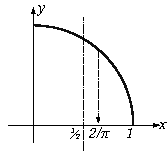
\includegraphics{05quartercircle.pdf}
  \caption{The average $x$-coordinate on a quarter circle}
  \label{fig:05average-x-on-quarter-circle}
\end{figure}

To compute these integrals we must first parametrize the curve.  Since the curve
is the unit circle, we can parametrize points on the curve by their polar
coordinate $\theta$, which gives us:
\[
\vx(t) = \vek \cos\theta \\ \sin\theta\tor \quad\text{and thus}\quad \|\vx'(t)\|
= \left\| \vek -\sin\theta\\ \cos\theta\tor\right \| = 1.
\]
Therefore
\[
\int_\cC x\; ds = \int_0^{\pi/2} \cos\theta \; d\theta =1.
\]
The length of the curve is $\pi/2$, so the average value of $x$ on the quarter
circle is
\[
\frac1{\pi/2} = \frac{2}{\pi} \approx 0.636\,619\,8\ldots.
\]

\section{Problems}

\begin{multicols}{2}\problemfont%
\problem If $\cC$ is the quarter of the unit circle that  lies in the first quadrant,
then\ldots

\subprob What is the average distance to the origin on $\cC$?  
\answer
The answer is 1.   You could compute that, but you don't have to.
The distance is 1 everywhere, so its average should also be $1$.
\endanswer
\subprob what is the average polar angle $\theta$? 
\answer
$\frac{\int_0^{\pi/2}\theta\; d\theta}{\pi/2} = \pi/4$
\endanswer

\problem 
\subprob Compute the average $x$ and $y$ coordinates of the polygon from $A(1,0)$ to $B(1,a)$ to $C(0,a)$ ($a>0$ is a constant; the polygon has the shape of an upside-down ``L'').

\subprob Compute the average polar angle $\theta$ on the same polygon $ABC$.

\problem Find the average $x$ and $y$-coordinates on the part that lies above the
$x$-axis of the circle with radius $R$ and center at the origin.
\answer
The average $x$ coordinate is zero, and the average $y$ coordinate is $2/\pi$.
\endanswer

\problem Compute $\int_\cC x\; ds$ where $\cC$ is the parabola $y=x^2$,  
with $0\le x\le 1$.
\answer
$\vx(t) = \tvek t \\ t^2\ttor$ is a parametrization, so the integral
becomes
\[
\int_\cC x\; ds
= \int_{t=0}^1 \underbrace{t}_{x=t} \; 
\underbrace{\sqrt{1+4t^2}}_{\|\vx'(t)\|} \; dt
=
\left[ 
\frac{2}{3}\frac{1}{8}\bigl(1+4t^2\bigr)^{3/2}
\right]_{0}^1
=\frac{5\sqrt{5}-1}{12}.
\]
\endanswer
\problem A wire is made in the shape of a helix,  of radius $a$ and height $H$, with
parametrization
\[
\vx(t) = \vek a\cos t \\ a\sin t \\ Ht/2\pi\tor\quad
(0\leq t\leq 2\pi).
\]
\begin{center}
  \begin{picture} (150.000000,176.428571)(0,0)
    \put(0.0, 0.0){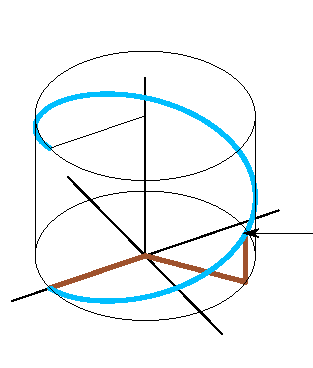
\includegraphics{05helix.pdf}}
        \put(  3.63,  30.11){\sffamily\itshape \makebox[0pt][r]{$x$}}
    \put(108.71,  14.19){\sffamily\itshape $y$}
    \put( 69.71, 141.38){\sffamily\itshape \makebox[0pt][c]{$z$}}
    \put( 70.71, 119.03){\sffamily\itshape \makebox[0pt][l]{$\tfrac{\pi}{2}$}}
    \put( 24.94,  42.32){\sffamily\itshape \makebox[0pt][c]{$1$}}
    \put( 97.14,  29.95){\sffamily\itshape \makebox[0pt][c]{$1$}}
    \put(148.00,  64.73){\sffamily\itshape \makebox[0pt][l]{$(\cos\theta, \sin\theta, \frac\theta4)$}}

\end{picture}

\end{center}
Suppose the temperature at $(x, y, z)$ is $T = T_0e^{-z/L}$ for constants
$L$ and $T_0$.

\subprob What are the units  of $a, H, T_0$, and $L$?
\answer
$a, H, L$ are lengths; $T_0$ is a temperature.
\endanswer
\subprob What values do $a$ and $H$ have  
for the helix in the drawing?
\answer
$a= 1$ is the radius of the cylinder on which the helix lies, and
$H=\pi/2$ is the height of one turn of the helix.
\endanswer
\subprob What is the average temperature on the wire? 
(Check that your answer has the right units.)
\answer
The average is 
\[
\text{average temp.  }=
\frac{\int_\cC T\; ds}{\int_\cC\; ds} .
\]
With the given parametrization $ds = \|\vx'(t)\|\; dt =
\sqrt{a^2 + H^2/4\pi^2}\; dt$ -- an ugly expression, but it's
constant, which is good for integrating.
You get
\[
\int_\cC ds = \int_0^{2\pi} \sqrt{a^2 + H^2/4\pi^2}\; dt
=2\pi\sqrt{a^2 + H^2/4\pi^2}=
\sqrt{4\pi^2a^2+H^2}.
\]
and
\begin{align*}
  \int_\cC T\; ds
  &= \int_0^{2\pi} T_0 e^{-Ht/2\pi L}\sqrt{a^2 + H^2/4\pi^2}\; dt\\
  &= T_0 \sqrt{a^2 + H^2/4\pi^2} \left[ -\frac{2\pi L}{H} e^{-Ht/2\pi L}
  \right]_{t=0}^{2\pi} \\
  &= T_0 \sqrt{a^2 + H^2/4\pi^2} \frac{2\pi L}{H} \left[ 1- e^{-H/L} \right].
\end{align*}
Therefore the average temperature is 
\[
\text{average temp.  }=
\frac{L}{H} \bigl(1-e^{-H/L}\bigr)\; T_0.
\]
\endanswer

\noproblemfont

\end{multicols}


\section{Line integrals of vector fields}

\subsection{Definition}
\label{sec:int-Fdx-def}\itshape
If $\cC$ is a curve in three dimensional space, and $\vF(x, y, z)$ is a vector
field, then the \emph{line integral of $\vF$ over $\cC$} is defined to be
\begin{equation}
  \int_\cC \vF\dpp d\vx = 
  \lim_{%
    \parbox{6em}
    {\footnotesize\sffamily
      \centering{``as the partition\\ gets finer''}}
  } \sum_{k=1}^n \vF(x_k, y_k, z_k) \dpp \Delta \vx_k
  \label{eq:05line-int-Fdx-def}
\end{equation}\upshape%
To define the Riemann sum we have partitioned the curve into $n$ pieces; $(x_k,
y_k, z_k)$ is a sample point on the $k^{\rm th}$ short arc in the partition, and
$\Delta \vx_k$ is the vector connecting the initial and final points of the
$k^{\rm th}$ partition arc.  See Figure~\ref{fig:05work-done-by-force} (right).


\subsection{Integrals over closed curves}
\label{sec:int-over-closed-curves}
A curve $\cC$ is \emph{closed} if its initial and final points coincide.  If we
are integrating a vector field over a closed curve, and if we want to emphasize
this in the notation, then we can write
\[
\oint_\cC \vF\dpp d\vx, \text{ or } \oint_\cC Pdx+Qdy+Rdz.
\]

\subsection{Differential form notation for line integrals}
\label{sec:form-notation}
The $d\vx$ that appears in line integrals is often interpreted as an
``infinitesimally short vector'' connecting two adjacent points on the curve
$\cC$.  Its components give us the amounts by which the coordinates $x, y$, and
$z$ change as we go ``from one point to the next'' on the curve, and therefore
one often writes
\[
d\vx = \tvek dx\\ dy\\ dz\ttor.
\]
If the vector field $\vF$ has components $\vF = \tvek P\\ Q \\
R\ttor$, where $P, Q$, and $R$ are functions of $(x,y,z)$, then the expression
$\vF\dpp d\vx$ can be written as
\[
\vF\dpp d\vx =\tvek P\\ Q \\ R\ttor \dpp\tvek dx\\ dy\\ dz\ttor
=P(x,y,z)dx+Q(x,y,z)dy+R(x,y,z)dz.
\]
Because of this the following notation for line integrals is often used:
\[
\int_\cC \vF\dpp d\vx = \int_\cC Pdx+Qdy+Rdz.
\]
For instance, the integral
\[
\int _\cC xdx+zdy-xydz
\]
stands for the line integral of the vector field $\vF = \tvek x\\ z\\
-xy\ttor$ over the curve $\cC$.

Expressions of the form $Pdx+Qdy+Rdz$, such as $x\,dx+z\,dy-xy\,dz$ above, are
called \emph{differential forms.}


% To define the ingredients of this Riemann sum you must first choose a
% parametrization $\vx(t)$ ($a \le t\le b$) of the curve.  Then you can
% partition the curve by partitioning the parameter interval into $n$ pieces,
% $a=t_0<t_1<\cdots<t_n=b$.  The $k^{\rm th}$ arc in the partition of the curve
% is $\{\vx(t), t_{k-1} \le t\le t_k\}$.  If the partition is very fine, then
% these arcs will be almost straight line segments.



\begin{figure}[t] 
  \centering
  \raisebox{36pt}{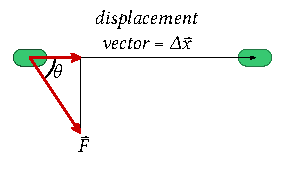
\includegraphics{05work.pdf}}
  \hspace{1in}
  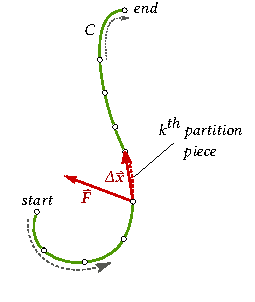
\includegraphics{05integral-of-vectorfield.pdf}
  \caption{\textbf{Left: } The work done by a force $\vF$ acting on an object is
    equal to the product of the length of the displacement $\Delta\vx$ and the
    magnitude of the force in the direction of the displacement.  If the angle
    between force and displacement is $\theta$, then this is $\mathcal{W} =
    \|\vF\|\|\Delta\vx\| \cos\theta = \vF\dpp\Delta\vx$.  \textbf{Right: } To
    define $\int_\cC\vF\dpp d\vx$ we partition the curve into small pieces, and
    add the work done by the force $\vF$ over all partition pieces.}
  \label{fig:05work-done-by-force}
\end{figure}

\subsection{The orientation of a curve}
\label{sec:05curve-orientation}
The Riemann sum (\ref{eq:05line-int-Fdx-def}) contains the vectors
$\Delta\vx_k$, which connect two adjacent points in our partition of the curve
$\cC$.  Whenever we have two points $A$ and $B$, there are \textit{two} vectors
connecting them, namely $\tpv AB$ and $\tpv BA = -\tpv AB$.  To make sure that
the direction of the vector $\Delta\vx_k$ in the Riemann sum
(\ref{eq:05line-int-Fdx-def}) is unambiguous, we have to agree on a direction in
which the curve $\cC$ is traversed.  Such a direction is called \emph{an
  orientation} of the curve.  A curve can have exactly two orientations, and to
distinguish between a curve and the same curve with the opposite orientation,
one writes
\[
-\cC = \textsf{the curve $\cC$ with its orientation reversed.}
\]
If one reverses the orientation of a curve (e.g.\ by switching its begin and end
points, see Figure~\ref{fig:05work-done-by-force}), then each vector
$\Delta\vx_k$ in the Riemann sum in (\ref{eq:05line-int-Fdx-def}) changes its
sign, and as a result the whole Riemann sum changes its sign.  In the limit the
integral changes its sign.  Thus we have
\begin{equation}
  \label{eq:05line-int-with-reversed-orientation}
  \int_{-\cC} \vF\dpp d\vx = - \int _\cC \vF\dpp d\vx.
\end{equation}
It is important to realize that the integral changes its sign here because it is
the line integral of a vector field.  If $w=f(x,y,z)$ is a function of three
variables then
\[
\int_{-\cC} f(x, y, z)\, ds = + \int_{\cC} f(x, y, z)\, ds.
\]
For instance, if $f=1$ is constant then $\int_{-\cC} ds$ and $\int_\cC ds$ are
the length of $-\cC$ and $\cC$.  Since the length of a curve is always a
positive number and does not depend on its orientation, we have
\[
\int_{\cC} ds = \text{length of }\cC = \text{length of }-\cC = \int_{-\cC} ds.
\]

\subsection{Integrating over piecewise defined curves}
To compute a line integral it is often best to start with a parametrization of
the curve and use~\eqref{eq:05line-integral-from-parametrization}.  In practice
it can be very difficult to find such a parametrization of the whole curve, even though
the curve can be broken into a few pieces, each of which does have a simple
parametrizations.  For instance, the edges of a square together form a closed
curve.  It is difficult to find one parametrization for all four edges at once,
but each edge of the square is a simple line segment for which one can easily
find a parametrization.
\begin{figure}[h]\centering
  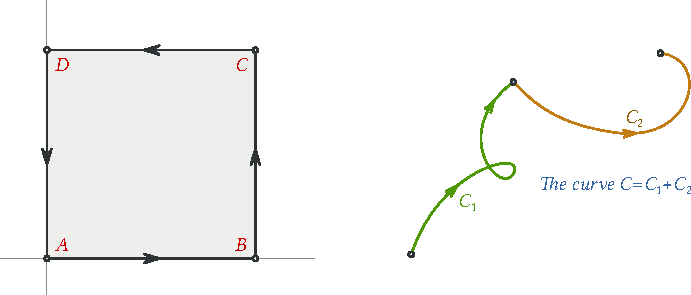
\includegraphics{05piecewise-defined-curve.pdf}
\end{figure}
In this situation one can write the line integral over the whole curve as a sum
of line integrals over the separate pieces.  Going back to the example of the
square, we have
\[
\int_{\cC}\vF\dpp d\vx = \int\limits_{AB}\vF\dpp d\vx + \int\limits_{BC}\vF\dpp
d\vx + \int\limits_{CD}\vF\dpp d\vx + \int\limits_{DA}\vF\dpp d\vx.
\]
In general, if a curve $\cC$ consists of two parts, $\cC_1$ and $\cC_2$, then we
express this by writing
\[
\cC = \cC_1 + \cC_2.
\]
A line integral over the whole curve is the sum of the line integrals over the
separate pieces:
\begin{equation}
  \int_\cC \vF\dpp d\vx = 
  \int_{\cC_1} \vF\dpp d\vx + 
  \int_{\cC_2} \vF\dpp d\vx .
  \label{eq:line-integral-over-broken-curve}
\end{equation}

\subsection{The line integral as the integral of the tangential component 
  of a vector field}
In the Riemann-sum (\ref{eq:05line-int-Fdx-def}) the $k^{\rm th}$ term contains
the vector $\Delta \vx_k$, which connects two adjacent points in the partition
of the curve (see figure~\ref{fig:05work-done-by-force}, on the right).  We can
write this vector as the product of a unit vector and a positive number:
\[
\Delta\vx_k = \frac{\Delta\vx_k}{\|\Delta\vx_k\|}\; \|\Delta \vx_k\|.
\]
The vector $\Delta\vx_k$ will be almost tangent to the curve, and the finer one
makes the partition, the smaller the angle between $\Delta \vx_k$ and the
tangent to the curve will be.  If the partition is sufficiently fine, then we
will have
\[
\frac{\Delta \vx_k}{\|\Delta\vx_k\|} \approx \vT_k,
\]
where $\vT_k$ is the unit tangent vector to the curve at the point $(x_k, y_k,
z_k)$.  Furthermore, $\Delta\vx_k \approx \Delta s_k$ approximates the length of
the $k^{\rm th}$ arc in the partition, and hence we can write the Riemann sum as
\[
\sum_{k=1}^n \vF(x_k, y_k, z_k) \dpp \Delta \vx_k \approx \sum_{k=1}^n \vF(x_k,
y_k, z_k) \dpp \vT_k \; \Delta s_k.
\]
The sum on the right is a Riemann sum for the line integral $\int_\cC
\vF(\vx)\dpp\vT\; ds$.  Taking the limit of arbitrarily fine partitions, we
conclude that
\begin{equation}
  \int_\cC \vF\dpp d\vx = \int_\cC \vF\dpp\vT\; ds.
  \label{eq:05line-int-of-tangential-part}
\end{equation}
Since $\vT$ is a unit vector, the quantity $\vF\dpp\vT$ is the length of
component of the vector field $\vF$ tangential to the curve.  Equation
\eqref{eq:05line-int-of-tangential-part} therefore says that the line integral
of the vector field $\vF$ along a curve $\cC$ is the same as the line integral
(in the sense of \S\ref{sec:line-integral-of-function}) of the tangential
component of $\vF$ along $\cC$.

\subsection{Example -- work around a circle}
\label{sec:work-around-the-circle}
The formula \eqref{eq:05line-int-of-tangential-part} for the line integral is
useful if we know the angle between the force $\vF$ and the curve, and the
magnitude of the force.  For instance, consider this problem:

\textit{Compute the work done by the vector field $\vF(x, y) = x\vi+y\vj = \tvek x\\
  y\ttor$ along the curve $\cC$, where $\cC$ is some piece of the unit circle in
  the plane.  }

\begin{figure}[h]
  \centering
  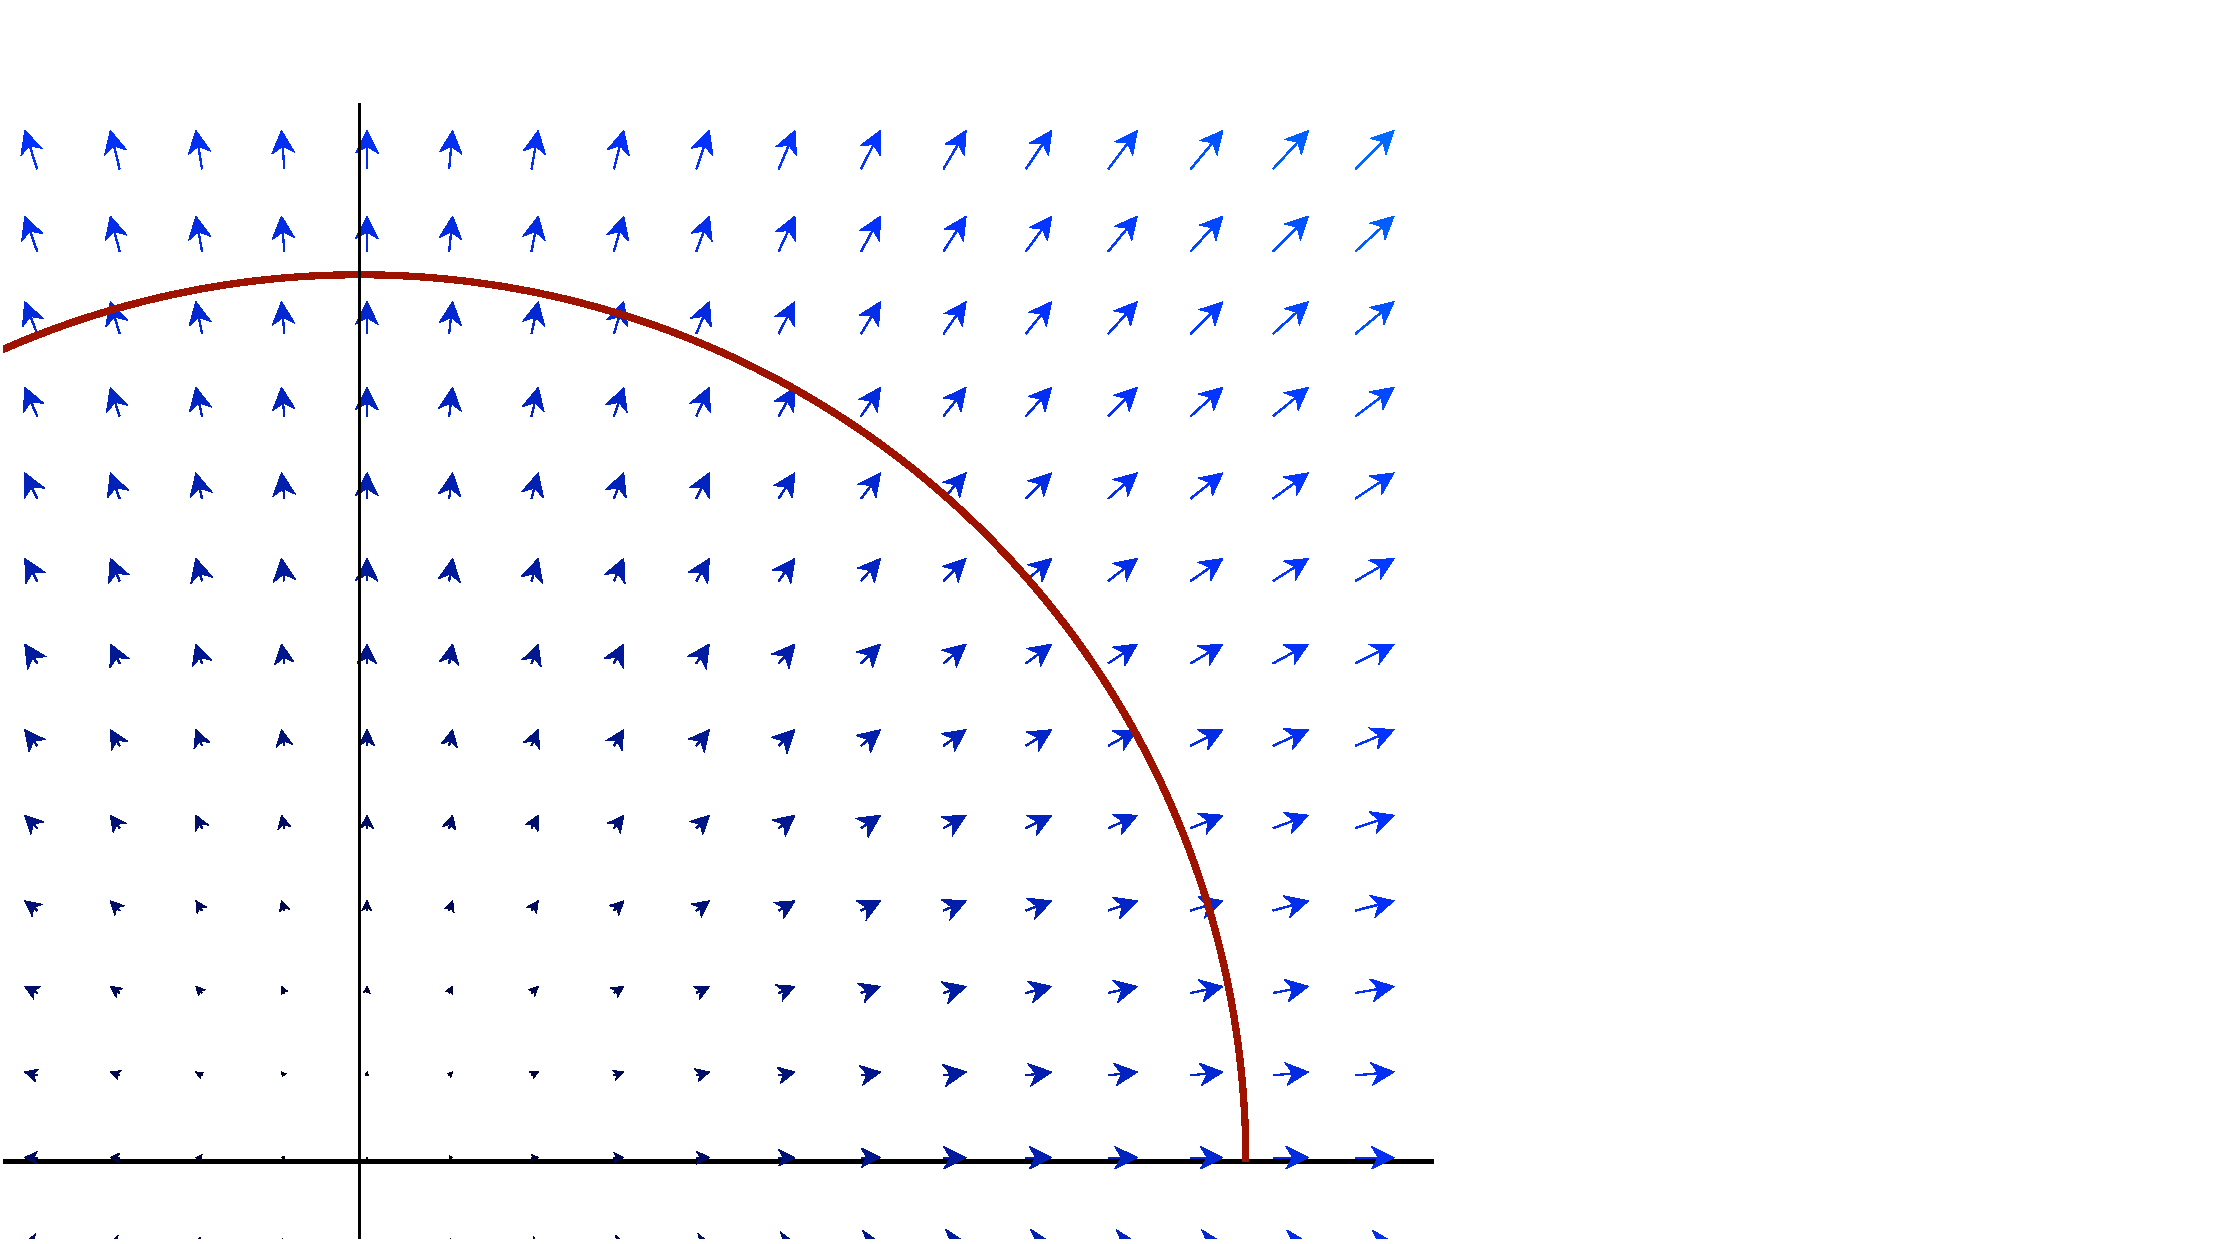
\includegraphics[width=0.4\textwidth]{05work-around-the-circle.pdf}\hspace{1in}
  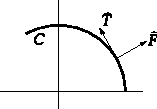
\includegraphics[scale=1.5]{05no-work-around-circlearc.pdf}
  \caption{\textbf{Left:} the vector field $\vF(x, y) = x\vi+y\vj$ from
    \S~\ref{sec:work-around-the-circle}.  \textbf{Right:} the vector field $\vF$
    is perpendicular to the path $\cC$ and hence does no work. }
  \label{fig:work-around-the-circle}
\end{figure}
We are asked to compute $\int_\cC\vF\dpp d\vx$.  The vector field $\vF = \tvek
x\\y\ttor$ always points away from the origin, and thus it is always
perpendicular to the tangent $\vT$ to the unit circle. (See
Figure~\ref{fig:work-around-the-circle}.)  Hence $\vF\dpp\vT = 0$, and we find
that
\[
\int_\cC \vF\dpp d\vx = \int_\cC \vF\dpp\vT \; ds = \int 0\; ds = 0.
\]
Those who prefer the differential form notation (\S~\ref{sec:form-notation}) can
write this as
\[
\int_\cC x\;dx+y\;dy = \int_\cC \vF\dpp d\vx = 0.
\]


\subsection{How to compute a line integral}
\label{sec:how-to-compute-int-Fdx}
If a parametrization of a curve $\cC$ is given, so that the curve $\cC$ is the
image of
\[
\vx = \vx(t) = \tvek x(t) \\ y(t) \\ z(t)\ttor, \quad a\leq t\leq b,
\]
then we can partition the curve $\cC$ by partitioning the parameter interval
$a\le t\le b$ by choosing partition points $a=t_0<t_1<\ldots<t_n=b$, just as in
\S\ref{sec:how-to-compute-int-fds}.  The $k^{\rm th}$ term in the Riemann sum
(\ref{eq:05line-int-Fdx-def}) defining $\int_\cC\vF\dpp d\vx$ is $\vF(x_k, y_k,
z_k)\dpp \Delta\vx_k$, with
\[
\Delta\vx_k = \vx(t_{k}) - \vx(t_{k-1}) \approx \vx'(t_k)\Delta t_k
\]
(again as in \S~\ref{sec:how-to-compute-int-fds}).  The Riemann sum for
$\int_\cC \vF\dpp d\vx$ is therefore
\[
\sum_{k=1}^n \vF(x_k, y_k, z_k) \dpp \Delta \vx_k \approx \sum_{k=1}^n \vF(x_k,
y_k, z_k) \dpp \vx'(t_k) \Delta t_k.
\]
The sum on the right converges to the integral $\int_a^b \vF(\vx(t))\dpp \vx'(t)
\; dt$, and thus we have found
\begin{equation}
  \label{eq:05int-Fdx-from-parametrization}
  \int_\cC \vF\dpp d\vx = \int_a^b \vF(x(t), y(t), z(t))\dpp \vx'(t) dt.
\end{equation}
We can think of this as a substitution formula for integrals, in which we
substitute $\vx = \vx(t)$ in the integral $\int_\cC \vF(\vx)\dpp d\vx$, using
the rule
\[
d\vx = \vx'(t) dt.
\]


\subsection{Three examples}
\label{sec:two-examples-of-work}
Let $\cC_1$ be the line segment from the origin to the point $(1,1)$, and let
$\cC_2$ be the piece of the parabola $y=x^2$ between the origin and the point
$(1,1)$.  Compute the work done by the vector field $\vF(x, y) = \tvek
-y\\x\ttor$ along each of these two paths.

The two curves $\cC_1$ and $\cC_2$ together bound a region $\cR$.  Let $\cC_3$
be the boundary of this region, traversed in clockwise direction, and compute
the work done by $\vF$ along the closed curve $\cC_3$.

\begin{figure}[h ]\centering
  \input ../figures/234/05there-two-ways.pdf_tex \input
  ../figures/234/05there-and-back.pdf_tex
  \caption{ \textbf{Left: } Two different paths from the origin to the point
    $(1,1)$, and the vector field $\vF$.  \textbf{Right: } By reversing the
    orientation of the second path $\cC_2$ we can create a closed path that
    starts and ends at the origin.  This path ($\cC_1$ combined with $-\cC_2$)
    is the boundary of the shaded region $\cR$, traversed in the
    \textit{clockwise} sense.}
\end{figure}


To find these integrals we need parametrizations of the curves.  For $\cC_1$ we
can use
\[
\vx_1 (t) = \vek t\\t\tor, \quad 0\leq t\leq 1,
\]
and for $\cC_2$ we can use
\[
\vx_2(t) = \vek t\\t^2\tor, \quad 0\leq t\leq 1.
\]
To show how both notations work, we will do the first integral using vector
notation, and the second using the differential form notation.

\subsubsection*{Integral over $\cC_1$}
The first integral is computed as follows:
\begin{align*}
  \int_{\cC_1} \vF\dpp d\vx &= \int_{\cC_1} \vek -y\\x \tor\dpp d\vx
  &&\text{substitute }\vx=\vx_1(t) = \vek t\\t\tor \\
  &= \int_{t=0}^1 \underbrace{\vek -t \\ t\tor}_{\vF} \dpp \underbrace{\vek
    1\\1\tor\; dt}_{d\vx}
  &&\text{since }d\vx = \vx_1'(t)dt = \vek 1\\1\tor dt\\
  &=\int_0^1 0\;dt\\[4pt]
  &=0.
\end{align*}
\subsubsection*{Integral over $\cC_2$}
The second integral written using differential forms is
\[
\int_{\cC_2} \vF\dpp d\vx = \int_{\cC_2} -y\;dx+x\;dy.
\]
Here we substitute the parametrization of the path
\[
x=x_2(t) = t\text{ and }y=y_2(t) = t^2,
\]
with
\[
dx = dt,\qquad dy = dt^2 = 2t\;dt,
\]
and we find
\[
\int_{\cC_2} \vF\dpp d\vx = \int_{t=0}^1 \underbrace{-t^2\;dt}_{-ydx} +
\underbrace{t\;2t\;dt}_{xdy} = \int_0^1 t^2\;dt =\frac13.
\]
\subsubsection*{Integral over $\cC_3$} We had defined $\cC_3$ to be the
combination of the curves $\cC_1$ and $-\cC_2$ (which is $\cC_2$ with its
orientation reversed).  Therefore
\begin{align*}
  \int_{\cC_3} \vF\dpp d\vx
  &=  \int_{\cC_1} \vF\dpp d\vx  + \int_{-\cC_2} \vF\dpp d\vx \\
  &= \int_{\cC_1} \vF\dpp d\vx - \int_{\cC_2} \vF\dpp d\vx .
\end{align*}
We have already computed these two integrals so there is no need to do a new
integration.  The result we are looking for is
\[
\int_{\cC_3} \vF\dpp d\vx = 0 - \frac{1}{3} = -\frac{1}{3}.
\]


\section[Another Fundamental Theorem]{Another Fundamental Theorem of Calculus}
If we know the derivative $f'(x)$ of a function $y=f(x)$ of one variable then
the Fundamental Theorem of Calculus tells us that we can recover the function by
integrating the derivative:
\begin{equation}
  f(b) = f(a) + \int_a^b f'(x)\,dx
  \label{eq:05fundamental-thm-one-variable}
\end{equation}
This semester we saw in chapter~IV, \S~\ref{sec:finding-f-from-its-derivs} that
one can do the same for functions of several variables, i.e.~following a
somewhat complicated procedure one can recover a function of two or more
variables if one knows it s partial derivatives.  In this section we show that
the procedure has a much shorter description in terms of a line integral.

\subsection{Theorem}\label{thm:fundamental}\itshape
For any path $\cC$ and any differentiable function $f$ one has
\begin{equation}
  f(B) - f(A) = \int_\cC \nab f(\vx)\dpp d\vx,
  \label{eq:05fundamental-thm-several-variables}
\end{equation}
where $A$ and $B$ are the initial and final points, respectively, of the path
$\cC$.  \upshape\medskip


In differential form notation the same statement is written as
\[
\int_\cC \left\{ \pdd fx \, dx +\pdd fy \, dy + \pdd fz \, dz \right\} =f(B) -
f(A).
\]

\subsection{Line integral of a gradient does not depend on the path}
The examples in \S~\ref{sec:two-examples-of-work} show that the line integral
$\int_\cC\vF\dpp d\vx$ of some vector field $\vF$ normally depends on the path
$\cC$.  However, it follows from Theorem~\ref{thm:fundamental} that if the
vector field $\vF$ happens to be the gradient of a function, $\vF=\nab f$, then
the line integral $\int_\cC \vF\dpp d\vx$ only depends on the initial and final
points, $A$ and $B$, of the path $\cC$, but not on the way that $\cC$ gets from
$A$ to $B$.


\subsection{Line integral of a gradient around a closed curve vanishes}
\label{sec:integral-over-closed-curve-of-gradient-vanishes}
An important special case of Theorem~\ref{thm:fundamental} is that in which the
curve $\cC$ is closed.  If $\cC$ is a closed curve, then its initial and final
points coincide, so that one always has
\begin{equation}
  \label{eq:05gradient-no-circulation}
  \oint_\cC \nab f(\vx)\dpp d\vx = 0.
\end{equation}


\subsection{Proof of the Fundamental Theorem}
Suppose $\vF = \nab f(x, y, z)$, and let the curve $\cC$ be parametrized by
$\vx=\vx(t)$, $a\le t\le b$.  Then
\[
\vF = \nab f = \vek f_x\\ f_y\\ f_z\tor,
\]
and hence
\begin{align*}
  \int_\cC\nab f \dpp d\vx
  &= \int_\cC \pdd fx dx +\pdd fy dy + \pdd fz dz \\
  &= \int_a^b \left\{
    \pdd fx(x(t), y(t), z(t)) \cdot x'(t)\right.\\
  &\hspace{4em} + \pdd fy(x(t), y(t), z(t))  \cdot y'(t)  \\
  &\left.  \hspace{6em} + \pdd fz(x(t), y(t), z(t)) \cdot z'(t) \right\} \;dt
\end{align*}
The expression between $\{\cdots\}$ is what the Chain Rule would give us if we
tried to differentiate $f(x(t), y(t), z(t))$ with respect to $t$.  So we get
\begin{align*}
  \int_\cC\nab f \dpp d\vx &=
  \int_a^b \frac{df(x(t), y(t), z(t))} {dt} \;dt \\
  &= f\bigl( x(b), y(b), z(b) \bigr) - f\bigl( x(a), y(a), z(a) \bigr).
\end{align*}
The point $B =(x(b), y(b), z(b)) $ is the end point of the curve $\cC$, and $A
=(x(a), y(a), z(a)) $ is its initial point, so we have found the fundamental
theorem~\eqref{eq:05fundamental-thm-several-variables}.  \bigskip

\begin{figure}[t]
  \input ../figures/234/05there-somehow.pdf_tex
  \caption{If we know the gradient of a function, and its value at one point
    (say, the origin), then we can compute $f(P)$ at any other point $P$ by
    choosing a path $\cC$ from the origin to $P$, and computing the line
    integral of the gradient.  We have $f(P) = f(0,0) + \int_{\cC} \nab f\dpp
    d\vx$.  It does not matter which path we choose.}
  \label{fig:05there-somehow}
\end{figure}

%%%%%%%%%%%%%%%%%%%%%%%%%%%%%%%%%%%%%%%%%%%%%%%%%%%%%%%%%%%%%%%%%%%%%%%%%%%
\section{Conservative vector fields}

\subsection{Definition}\label{sec:conservative-vector-fields}\itshape
A vector field $\vF$ is called \emph{conservative} if one has
\begin{equation}
  \oint_\cC \vF\dpp d\vx = 0
  \label{eq:conservative-because-no-work}
\end{equation}
for every closed curve $\cC$.\upshape

The name ``conservative'' derives from the interpretation of the integral
in~\eqref{eq:conservative-because-no-work} as the amount of work done by the
force field $\vF$ around the closed curve $\cC$.  As an object moves throughout
the plane along the curve $\cC$, the force $\vF$ acts on it, does work, and
therefore provides energy to the object.  The line integral
\eqref{eq:conservative-because-no-work} measures how much energy the force adds
to the object after going around the curve $\cC$ once.  For a conservative
vector field the total energy provided to the object is exactly zero, suggesting
that its energy is \emph{conserved}.
\begin{figure}[h]
  \input ../figures/234/05work-around-any-closed-curve.pdf_tex
  \caption{As an object moves along the closed curve $\cC$ the force $\vF$ acts on
  it.  At times the force works in the direction of the motion, at other times it
  works against the motion.  If the object starts at $P$, and goes around once, will
  it have gained energy when returning to $P$?}
  \label{fig:05work-around-any-closed-curve}
\end{figure}

It follows from \S~\ref{sec:integral-over-closed-curve-of-gradient-vanishes}
that any vector field $\vF$ that is the gradient of a function is a conservative
vector field.  The following theorem says that these are actually the only
conservative vector fields.

\subsection{Theorem}\itshape If $\vF$ is a conservative vector field then there is a
function $f$ such that $\vF = \nab f$.\upshape \medskip

If $\vF=\nab f$ the function 
\[
  V = -f
\]
is called a \emph{potential} of the vector field $\vF$.  Thus a function $V$ is a
potential of the vector field $F$ if
\[
  \vF = -\nab V.
\]
The potential $V$ can be found by choosing one fixed point $A$, at which we declare
$V(A)=0$, and then computing the line integral
\begin{equation}
  V(P) \stackrel{\rm def}= -\int_A^P \vF\dpp d\vx
  \label{eq:potential-found}
\end{equation}
where the integral is a line integral over a path from the point $A$ to the
point $P$.  The assumption that $\vF$ is a conservative vector field implies
that the integral in \eqref{eq:potential-found} does not depend on the path that
is chosen.
% TO DO : include proof.

\newpage
\section{Problems}
\begin{multicols}{2}
\problemfont

\problem Is the gravitational vector field
\[
  \vg(x, y) = -g\ves2 = \tvek 0 \\ -g\ttor
\]
a conservative vector field?
\answer
Yes.  It is the gradient of $f(x, y) = gy$.
\endanswer

\problem Newton's gravitational vector field
\[
  \vF(x, y) = -\frac{\vx}{\|\vx\|^3}
\]
from \S\ref{sec:force-field-examples}, equation~\eqref{eq:05Newton-on-gravity} is a
conservative vector field.  Show this by finding a potential of the form $f(x, y, z)
= K\|\vx\|^a$ for suitable constants $a$ and $K$.

\problem Reread the section in Chapter~IV about Clairaut's theorem.  You now have two
ways to tell that a vector field $\vF = P(x, y)\ves1 + Q(x, y)\ves2$ cannot be a
gradient.  Which are they?
\answer
By Clairaut's theorem, if $\vF$ is a gradient, then $P_y = Q_x$.

By the fundamental theorem for line integrals, if $\vF$ is a gradient, then
$\oint_\cC \vF\dpp d\vx =0$ (or, equivalently, $\oint_\cC Pdx+Qdy=0$) for every
closed curve $\cC$.
\endanswer


\problem  % Compute the line integrals of F and G over the unit circle
\subprob Compute the line integrals of the vector fields
\[
 \vF = \vek  x\\0 \tor \quad\text{and}\quad
 \vG = \vek 0\\x \tor 
\]
around the unit circle $\vx(\theta) = \cos\theta\ves1 + \sin\theta\ves2$.
\answer
$\int_\cC \vF\dpp d\vx = \int_\cC xdx = 0 $.

$\int_\cC \vG\dpp d\vx = \int_\cC xdy = \pi$.
\endanswer


\subprob Which of the vector fields $\vF$ or $\vG$ \emph{cannot} be a gradient, based on your answer to \textbf{(a)}?
\answer
Since $\int_\cC \vG\dpp d\vx \neq0$ the vector field $\vG$ cannot be a gradient.
\endanswer


\subprob Can you conclude from your answer to \textbf{(a)} that any of the vector
fields $\vF$ or $\vG$ must be a gradient?
\answer
The integral $\int_\cC\vf\dpp d\vx$ vanishes, but to check that $\vF$ is conservative
one has to check $\int_\cC\vf\dpp d\vx =0 $ for \emph{all} closed curves $\cC$, and
not just the unit circle.  So our integral computation does not imply that $\vF$ is a
gradient.

You can use different arguments to show directly that $\vF$ is a gradient, for
instance, by noting that $\nab (\frac12 x^2) = \tvek x\\0 \ttor$, or if you're not
that lucky, by using the methods of \S~IV.\ref{sec:finding-f-from-its-derivs}.
\endanswer


\noproblemfont

\end{multicols}
\section{Flux integrals}
\label{sec:flux-integrals}
\subsection{Definition of flux}
In \S~\ref{sec:int-Fdx-def} we defined the integral of a vector field along a
curve $\cC$ as the line integral of the tangential component of the vector
field.  If the curve $\cC$ is not a space curve, but lies in the $xy$-plane,
then one can also define the \emph{flux of the vector field across the curve}.

To define the flux we must first choose a unit normal vector $\vN$ for the curve
$\cC$, i.e.~at each point on $\cC$ we must choose a vector $\vN$ that has unit
length and that is perpendicular to the curve:
\[
\|\vN\|=1, \quad\text{and}\quad \vN\dpp\vT = 0.
\]
Once a unit normal for the curve $\cC$ has been chosen, the flux of a vector
field $\vv$ across the curve $\cC$ in the direction of $\vN$ is defined to be
\begin{equation}
  \textsf{Flux}
  =
  \int_\cC \vv\dpp\vN\, ds	
  \label{eq:flux-defined}
\end{equation}

\begin{figure}[ht]
  \input ../figures/234/05flux.pdf_tex
  \caption{ \textbf{Left:} At each point on a plane curve there are two choices of
  unit normal.  If a unit tangent is given, then the most common choice of normal is
  to rotate the unit tangent counterclockwise by $90^\circ$.\\
    \null\quad%
    \textbf{Top, right:}  if water is flowing over the plane with velocity field $\vv$, then the rate at which water flows across the curve $\cC$ in the direction of the normal $\vN$ is given by the flux integral~\eqref{eq:flux-defined} of the velocity.\\
    \null\quad%
    \textbf{Bottom, right:} the amount of water flowing across a short arc of
    length $\Delta s$ on the curve $\cC$ in time $\Delta t$ is the area of a
    parallelogram one of whose sides is $\vv\Delta t$.  The area of this
    parallelogram is the length of the normal component of $\vv\Delta t$ times
    $\Delta s$.}
  \label{fig:flux-across-C}
\end{figure}

The flux integral has a very natural interpretation if the vector field $\vv$ is
the velocity field of a two dimensional fluid flowing in the plane.  If $\cC$ is
an arc in the plane, and if $\vN$ is a unit normal to $\cC$, then fluid will
flow across this arc, and one can ask how much fluid flows across the arc in the
direction of $\vN$.  The answer is given by the flux
integral~\eqref{eq:flux-defined}.  For an explanation see
Figure~\ref{fig:flux-across-C}.  There the arc is divided into many small sub
arcs, which may be considered nearly straight.  During a time interval of length
$\Delta t$ the fluid flowing through one such short arc sweeps out a
parallelogram of which one side has length $\Delta s$, while the other is given
by the vector $\vv\Delta t$.  The area of the small parallelogram is then
$\vN\dpp\vv \Delta t\, \Delta s$.  To get the rate at which fluid flows across
the short arc we divide this by $\Delta t$ to get $\vv\dpp\vN \Delta s$.  Adding
over all short arcs that comprise the curve $\cC$ leads to the flux
integral~\eqref{eq:flux-defined}.

\subsection{Flux across a closed curve}
\label{sec:flux-across-a-closed-curve}
If $\cC$ is a closed curve without self intersections, and $\cR$ is the region
it encloses then the flux of a vector field $\vv$ across the curve $\cC$ can
again be interpreted as the rate at which fluid flows across the curve $\cC$.
Since the curve now encloses the bounded region $\cR$, we can also say that the
flux of $\vv$ across the curve $\cC$ is the net rate at which fluid leaves the
region $\cR$ (provided $\vN$ is the outward pointing unit normal).
\begin{figure}[h]
  \centering
  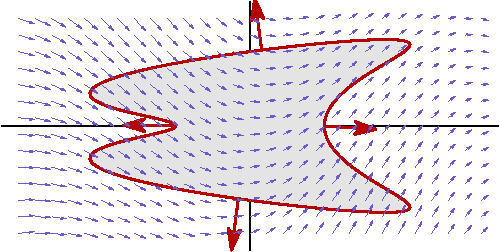
\includegraphics[scale=0.8]{05flux-across-closed-curve.pdf}
  \caption{The flux of a vector field $\vv$ across a closed curve measures the rate
    at which fluid is flowing out of the enclosed region, if $\vN$ is the
    \textit{outward} normal to the curve.}
\end{figure}

% \subsection{Differential form version of the flux integral}
%
%
%\begin{figure}[h]
%  \input ../figures/234/05flux-line-element.pdf_tex
%\end{figure}


\subsection{Example -- water under the bridge}
An endless river $\cR$ occupies the strip
\[
\cR = \{(x,y) : -1\leq y \leq 1\}
\]
in the $xy$-plane.  (The width of the river is $2$.)  The water in the river
flows with velocity
\[
\vv(x, y) = V(1-y^2) \ves1 = \vek V(1-y^2)\\0\tor,
\]
where $V$ is a constant (it is the maximal velocity of the water, which is
attained at $y=0$, i.e.~in the middle of the river; this flow is a two dimensional version of the Poiseuille flow from \S~\ref{sec:fluid-flow}.)

\subsubsection*{Question:}\itshape How much water flows from left to right through
the line segment $AB$, where $A$ is the point $(0,-1)$, and $B$ is the point
$(0,1)$?  \upshape

\subsubsection*{Solution:} We parametrize the line segment by
\[
\vx(u) = \vek 0\\u\tor, \quad -1\leq u\leq1.
\]
Normally one refers to the parameter as ``time,'' but since we are considering
flowing water, time is already part of the problem.  Therefore we have called
the parameter on the curve $u$ instead of $t$.

The line segment is vertical, so the unit normal is a horizontal vector of
length 1, i.e.~either $\vN=\ves1$ or $\vN=-\ves1$.  We are asked to find how
much water flows \textit{from left to right}, so we need the normal that points
to the right: $\vN=+\ves1$.

\begin{figure}[t]
  \input ../figures/234/05flux-example1.pdf_tex
  \caption{The shaded region represents the water that passed under the bridge
    during one time unit.}
\end{figure}

We can now compute the integral.  We begin with
\[
ds = \|\vx'(u)\| du = \left\|\vek 0\\1\tor \right\|\,du = du,
\]
and
\[
\vN\dpp\vv = \vek 1\\0\tor \dpp \vek V(1-y^2)\\0\tor = V(1-y^2) = V\bigl(1-
u^2\bigr),
\]
which gives us
\[
\int_\cC\vv\dpp\vN\,ds = \int_{u=-1}^1 V(1-u^2) du =V[u-\tfrac13u^3]_{-1}^1
=\tfrac43 V.
\]

\subsection{An expanding flow}
\label{sec:expanding-flow-example}
A substance, perhaps a fluid, or a gas, is spreading from the origin and is
moving with velocity field
\[
\vv = V \vek x/R\\ y/R \tor =\frac{V} {R}\, \vx,
\]
where $V$ and $R$ are constants: $V$ has the units of a velocity, and $R$ has
the units of a length.  The interpretation of these constants is that $V$ is the
speed at which fluid particles are moving when they are at a distance $R$ from
the origin.

\begin{figure}
  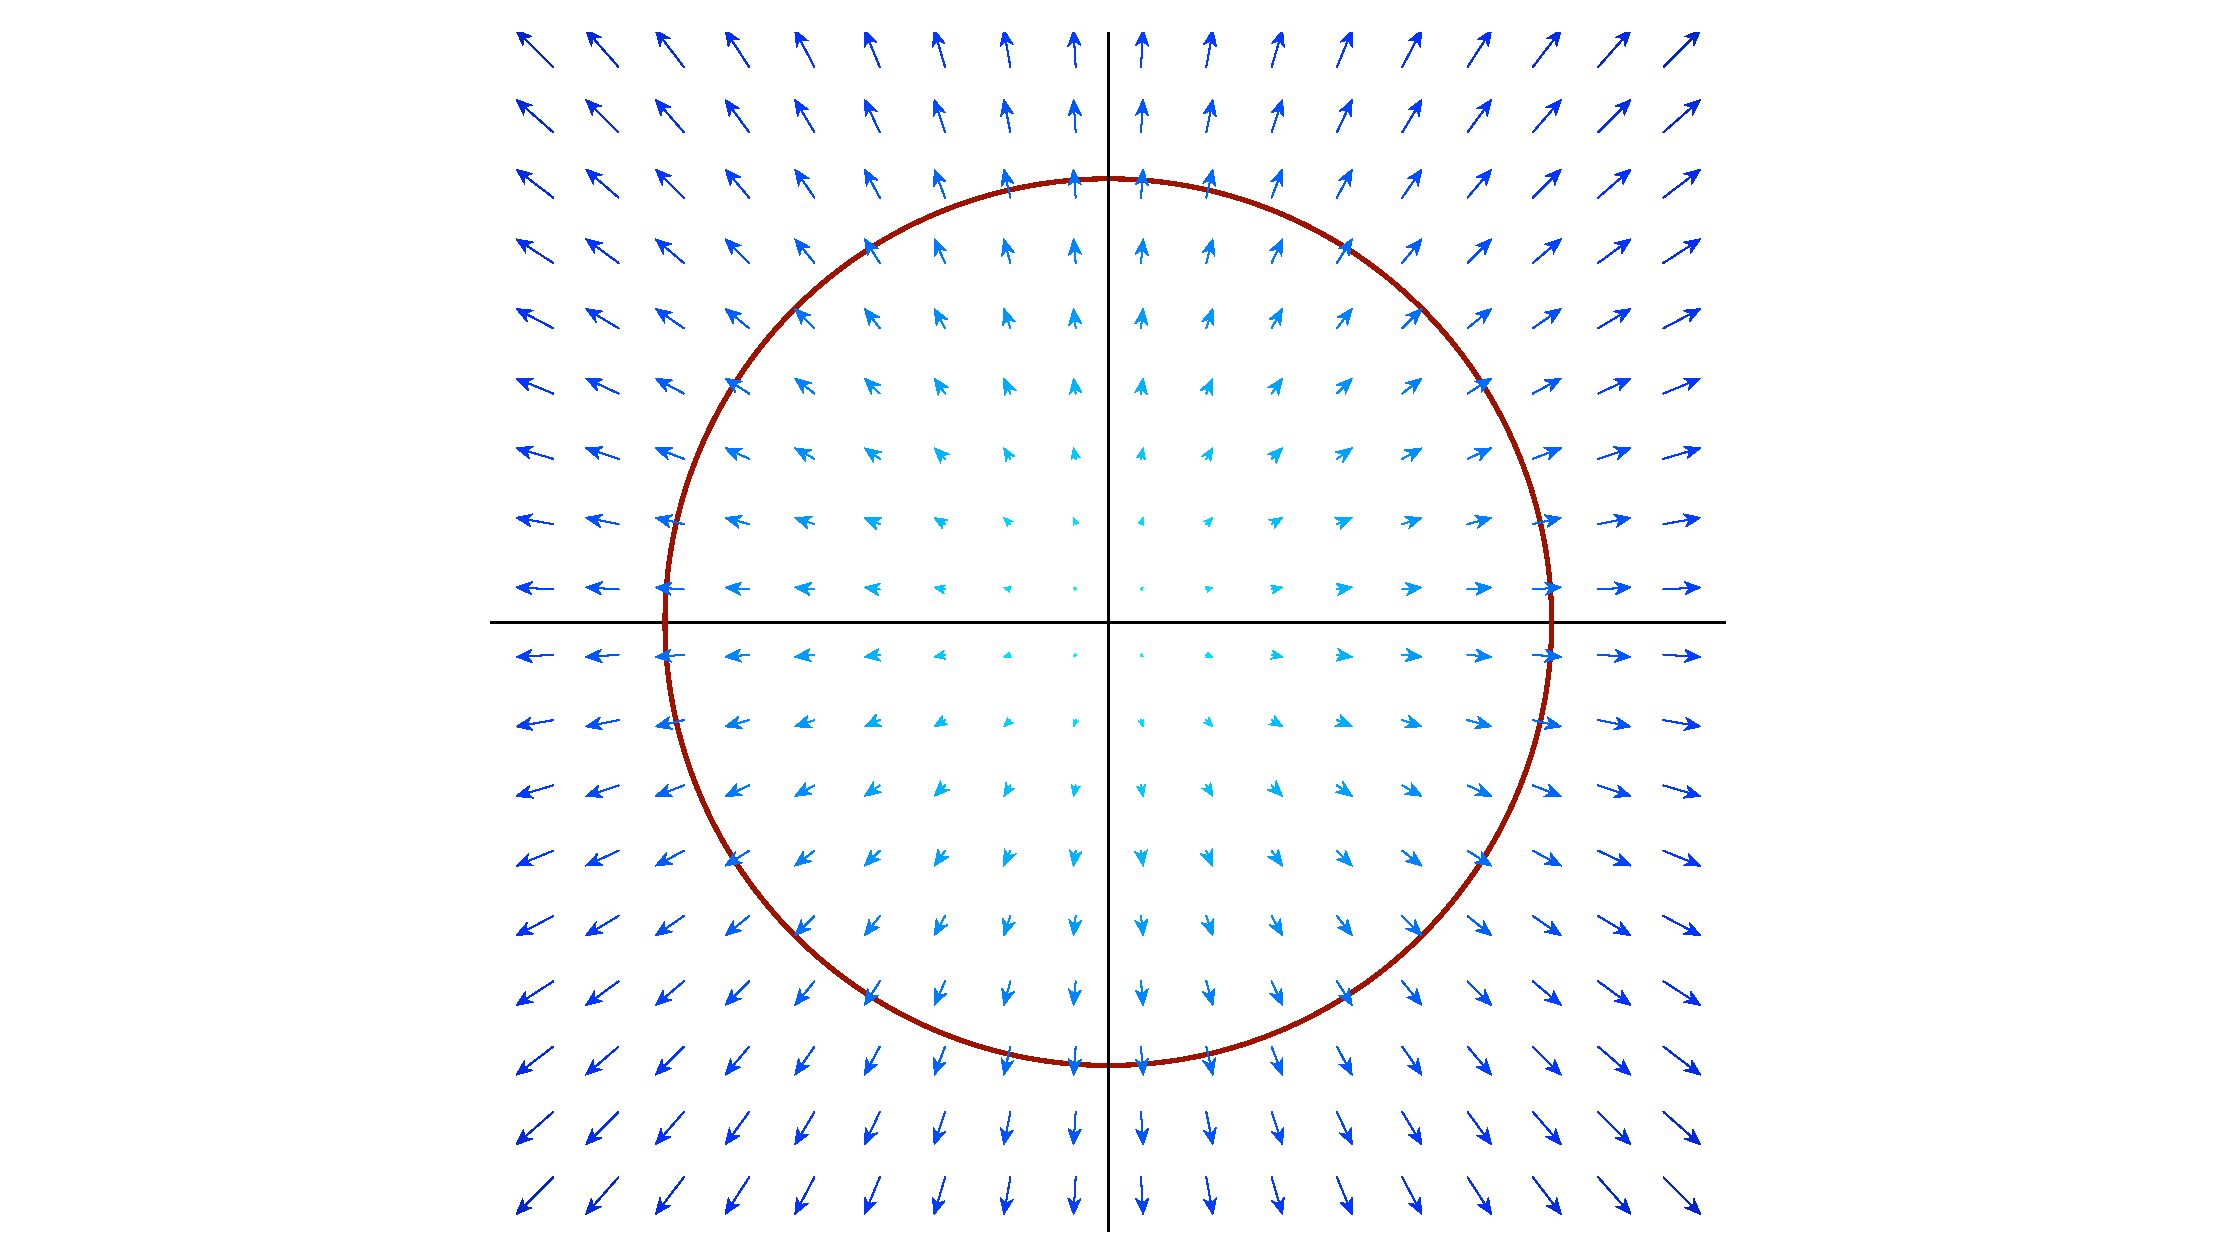
\includegraphics[width=0.4\textwidth]{05expanding-fluid.pdf}
  \qquad
  \raisebox{12pt}{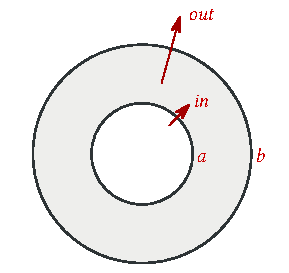
\includegraphics{05expanding-fluid-through-annulus.pdf}}

  \caption{\textbf{Left: }The vector field $\vv(x,y) = \frac{V}
    {R}\bigl(x\ves1+y\ves2\bigr)$ and a circle with radius $a$.  \textbf{Right:
    } This vector field cannot describe the flow of an ``incompressible'' fluid
    like water since more fluid flows out of the circle with radius $b$ than
    through the circle with radius $a$: water would have to be created in the
    annular region between the two circles.}
\end{figure}

\noindent%
\subsubsection*{Question:}\itshape How much fluid flows out of the circle with radius
$a$?  \upshape\smallskip

Before we compute anything let us decide on the units that the answer should
have.  The question of ``how much'' fluid flows across the curve is ambiguous
since we could answer in terms of mass (pounds or kilograms of fluid per
second), or in terms of volume (gallons per second).  These two are related by
the density (pounds per gallon, kilos per liter, etc.) of the substance, and
since we do not know anything about the density we will measure ``how much'' in
terms of the volume of substance flowing across the curve per second.  In fact,
since we are dealing with a two dimensional model (the substance is flowing in
the plane rather than three dimensional space, we will measure the area that
flows across the curve instead of the volume.

\subsubsection*{Solution:} We need to compute
\[
\oint_{\cC_a} \vv\dpp\vN\, ds
\]
where $\cC_a$ is the circle with radius $a$ centered at the origin.  The unit
normal $\vN$ is the outward pointing normal, because we are asked to find how
much fluid flows \textit{out} of the circle.

In this case $\vN$ and $\vv$ are parallel so that on the circle $\cC_a$ we have
\[
\vN\dpp\vv = \|\vv\| = V\frac aR.
\]
Therefore the flux integral is very simple, namely
\[
\oint_{\cC_a} \vv\dpp\vN\, ds = \oint_{\cC_a} V\frac aR ds = V\frac aR
\cdot\underbrace{\oint_{\cC_a}ds}_{\textsf{Length of $\cC_a$}} = 2\pi
\frac{Va^2}{R}.
\]
This answer is unrealistic if we assume that $\vv$ really is the velocity field
of a normal fluid (like water).  To see what is wrong we compute how much fluid
flows through circles of different radii $a$ and $b$.  If $a<b$ then the rate at
which fluid flows through the smaller circle is less than the rate at which
fluid flows out of the larger circle.  The difference,
\begin{equation}
  \frac{2\pi V}{R} \bigl(b^2-a^2\bigr),
  \label{eq:fluid-production-in-annulus}
\end{equation}
represents the amount of fluid that is (apparently) being created every second
in the ring-shaped region between $\cC_a$ and $\cC_b$.

However, the computation could apply to a flowing gas.  In this case we have
computed the volume of gas that flows across each circle per time unit (or the
area of gas, because we are using a two dimensional model here).  A larger
volume could flow across $\cC_b$ than across $\cC_a$, provided the gas is less
dense at the circle $\cC_b$ than it is at the smaller circle $\cC_a$.  This kind
of reasoning is important for fluid and gas dynamics, and in fact appears in
many other branches in physics.



\section{Green's Theorem}
We have seen that the line integral $\oint_\cC \vF\dpp\vT\, ds$ of a vector
field along a closed curve vanishes if the vector field happens to be the
gradient of some function
(\S~\ref{sec:integral-over-closed-curve-of-gradient-vanishes}), but if the
vector field $\vF$ is not the gradient of a function then its line integral
around a closed curve need not vanish (see the example in
\S~\ref{sec:how-to-compute-int-Fdx}).  We have also seen examples where a flux
integral $\oint_\cC \vv\dpp\vN\, ds$ is non-zero.

Green's theorem relates the line integral of any vector field on the boundary
curve $\cC$ of some domain $\cR$ with a double integral involving partial
derivatives of the vector field on the domain $\cR$ itself.  There are two
versions of the theorem, depending on what kind of line integral one considers.
The first version is for ``work-type integrals,'' and is best written in
differential form notation.  The second version is about flux integrals.

\subsection{Simply connected domains}
\label{sec:simply-connected-domains}
In both versions of Green's theorem one has a plane region $\cR$ and its
boundary curve(s).  The boundary curves of a region can be somewhat complicated.
The simplest situation is where the domain $\cR$ is \emph{simply connected.}
This means that $\cR$ is the region enclosed by \textit{one} curve $\cC$ (the
curve $\cC$ is not allowed to intersect itself.)  Another way of describing what
a simply connected region is, is to say that a region is simply connected if
``it has no holes.''  See Figure~\ref{fig:simply-and-not-simply-connected}.  If
a domain is not simply connected, then its boundary may consist of more than one
curve (Figure~\ref{fig:simply-and-not-simply-connected} on the right).

\subsection*{Green's theorem}\itshape%
Let $\cR$ be a simply connected region in the plane, and let $\cC$ be the
boundary curve of the region $\cR$, with the counter clockwise orientation.  Let
\[
\vv(x,y) = P(x,y)\ves1 + Q(x,y)\ves2
\]
be a vector field that is defined and has
continuous derivatives \emph{everywhere} in $\cR$.  Then one has\upshape
\begin{equation}
  \oint_\cC P(x,y) dx + Q(x, y) dy = 
  \iint\limits_\cR \left\{
    \pdd Qx - \pdd Py
  \right\} \; dA.
  \label{eq:Greens-thm}
\end{equation}

\begin{figure}
  \input ../figures/234/05domain-with-boundary.pdf_tex
  \caption{\textbf{Left: } A simply connected domain, i.e.~ a domain``without
    holes.''  \textbf{Right:} a non-simply connected domain, i.e.~``a domain
    with a hole.''  For this non-simply connected domain the boundary consists
    of two closed curves rather than one.}
  \label{fig:simply-and-not-simply-connected}
\end{figure}

The second form of Green's Theorem is about flux integrals and is often called
the ``\emph{divergence theorem.}''
\subsection*{Flux version of Green's theorem}\itshape%
Let $\cR$ be a bounded domain in the plane that is enclosed by a curve $\cC$.
If
\[
\vv = \vek P(x,y)\\ Q(x,y) \tor
\]
is a vector field that is everywhere defined and differentiable on $\cR$,
then
\begin{equation} 
  \oint_\cC \vv\dpp\vN\,ds = \liint_\cR \Bigl\{\pdd {P}x +
  \pdd {Q}y\Bigr\}\,dA
  \label{eq:divergence-theorem-plane}
\end{equation}
where $\vN$ is the outward unit normal for the domain $\cR$. \upshape\medskip

The quantity
\begin{equation}
  \pdd {P}x + \pdd {Q}y
  \label{eq:divergence-of-plane-vector-field}
\end{equation}
is called the \emph{divergence} of the vector field $\vv$, and is written as
``$\div \vv$.''  It is one of several combinations of partial derivatives of vector fields that turn out to be useful.  See \S~\ref{sec:nabla} for more of these.


\subsection{Examples illustrating Green's Theorem}

\subsubsection*{An example where the line integral vanishes on any closed curve}
Consider the vector field
\[
\vF(x, y) = x\ves1 + y\ves2 = \tvek x\\y \ttor,
\]
and let $\cC$ be a closed curve in the plane, that encloses the region $\cR$.
Then the line integral of $\vF$ along $\cC$ is given by
\begin{align*}
  \oint_\cC \vF\dpp d\vx
  &= \liint_{\cR} \bigl\{ \pdd yx - \pdd xy\bigr\} \;dA \\
  &= \liint_{\cR} 0 \;dA\\
  &= 0.
\end{align*}
We find that the integral is always zero, no matter what the region $\cR$ is.
If we were lucky enough to note that this particular vector field is a gradient,
\[
\vF = \vek x\\y \tor = \nab \bigl( \tfrac12 x^2 +\tfrac12 y^2\bigr),
\]
then we could also have used~\eqref{eq:05gradient-no-circulation} to conclude
that $\oint _\cC \vF\dpp d\vx =0$ for any closed curve $\cC$.
\subsubsection*{The expanding gas example again} Let
\[
\vv(x, y) = \frac{V}{R}\vx = \frac{V}{R}x\ves1 + \frac VR y\ves2
\]
be the velocity field of the expanding gas from
\S~\ref{sec:expanding-flow-example}, and let $\cC$ be any closed curve that is
the boundary curve of some domain $\cR$.  We again compute the flux of the
velocity field across the curve $\cC$ in the direction of its outward normal,
but this time we use Green's Theorem.

\begin{figure}[h]
  \begin{minipage}[b]{0.6\textwidth}
    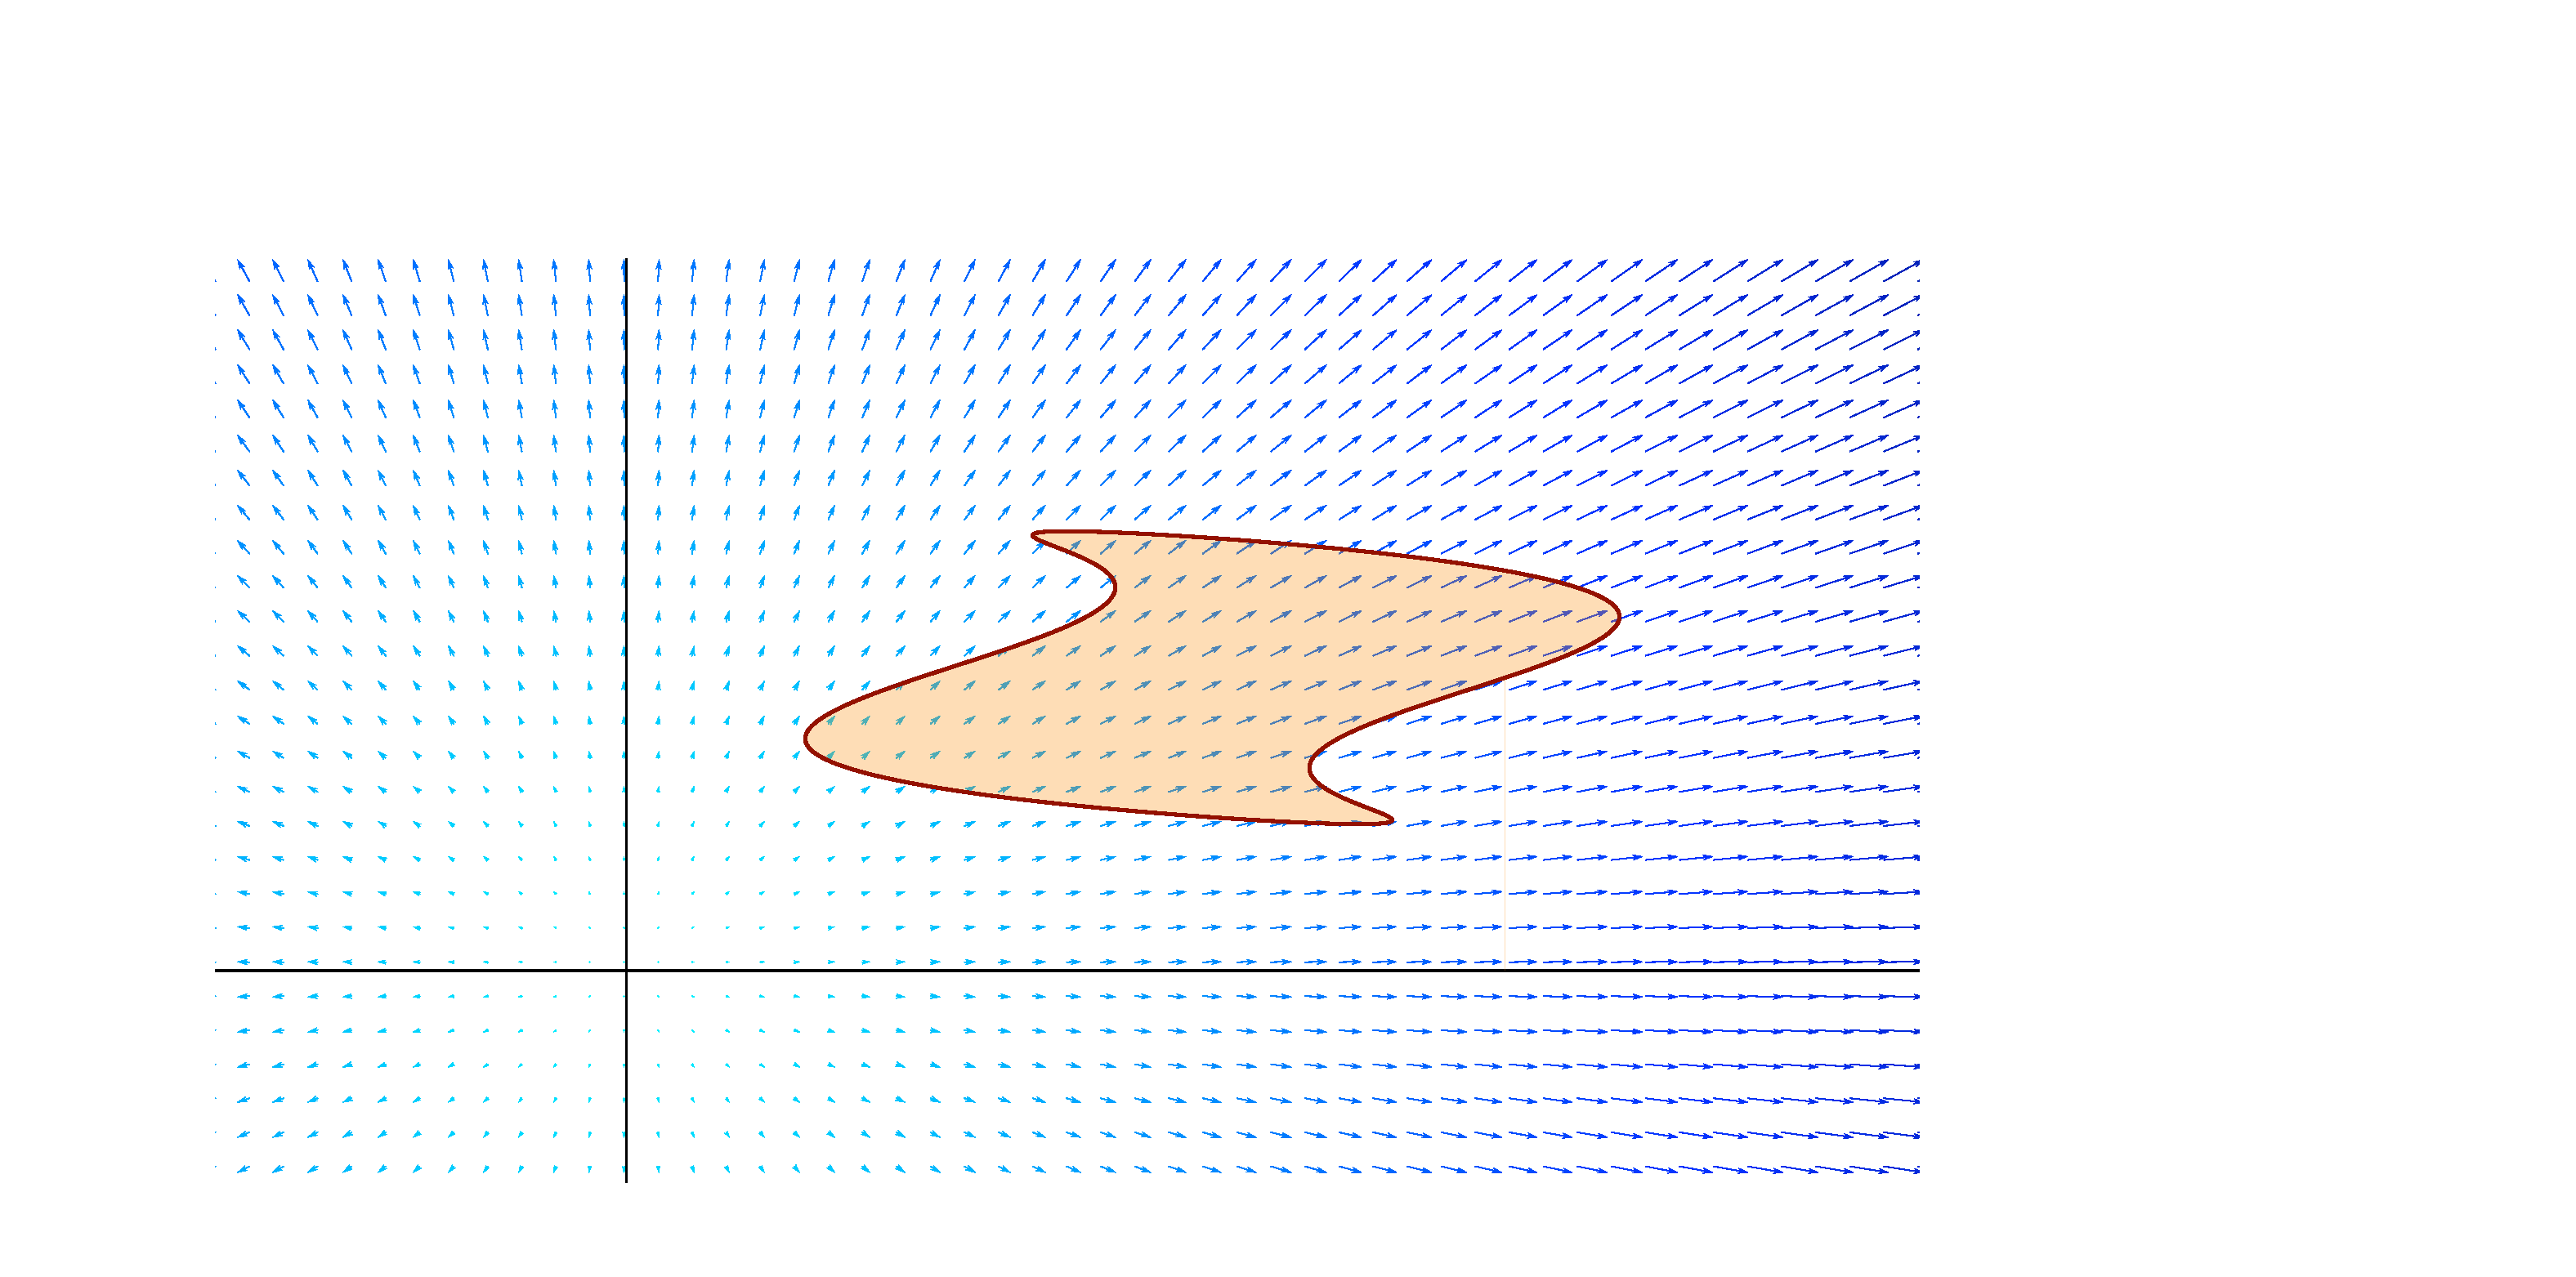
\includegraphics[width=\textwidth]{05expanding-fluid2.pdf}
  \end{minipage}\hfill
  \begin{minipage}[b]{0.3\textwidth}
    \caption {A ``gas'' is flowing in the plane with velocity field $\vv$.
    At what rate is gas flowing out of the shaded region?\\
    \null\quad The answer turns out to be proportional to the area of the region.\\
%    \rule{0pt}{18pt}
}
    \label{fig:05expanding-fluid2}
\end{minipage}
\end{figure}%

According to Green's Theorem we have
\[
\oint_\cC \vv\dpp\vN \, ds = \liint_\cR \div\vv\, dA
\]
where $\div \vv$ is the divergence of $\vv$, defined in
\eqref{eq:divergence-of-plane-vector-field}.  Thus
\[
\div \vv = \pdd{v_1}x + \pdd{v_2}y =\pdd {\{Vx/R\} }x + \pdd {\{Vy/R\}}y =\frac
VR + \frac VR =2\frac VR,
\]
and finally,
\begin{equation}
  \oint_\cC \vv\dpp\vN \, ds
  =
  \liint_\cR 2\frac VR\,dA = 2\frac VR\cdot\textsf{area of $\cR$}.
  \label{eq:fluid-production-in-any-region}
\end{equation}
This is consistent with our previous computation in
\S~\ref{sec:expanding-flow-example}.  There we found
in~\eqref{eq:fluid-production-in-annulus} that the amount of fluid produced in
an annulus of inner and outer radii $a$ and $b$ is $2\pi \frac VR(b^2-a^2)$.
Since the area of the annulus is $\pi b^2 - \pi a^2$ this is the same result
that we just found in \eqref{eq:fluid-production-in-any-region}.

\section{Conservative vector fields and Clairaut's theorem}
\label{sec:clairaut-is-conservative}
Let $\vF(x, y) = P(x, y)\ves1 + Q(x,y)\ves2$ be a vector field on some region
$\cR$ in the plane.  The fundamental theorem for line integrals and Clairaut's
Theorem (III.\ref{thm:Clairaut}) provide connections between conservative vector
fields, gradient vector fields, and the partial derivatives of $P$ and $Q$.  To
summarize what we have seen so far, recall that\dots
\begin{itemize}
  \itshape
\item if $\vF = \nab f$ for some function $f(x,y)$ then $\vF$ is conservative,
\item \rule{0pt}{14pt}%
  if $\vF$ is conservative then $\vF = \nab f$ for some function $f(x,y)$
\item \rule{0pt}{18pt}%
  if $\vF = \nab f$, then $\DS \pdd Py = \pdd Qx$.
\end{itemize}
Looking at this list we see that the missing statement would be that ``$P_y =
Q_x$ implies that $\vF$ is a gradient vector field.''  This turns out only to be
true if we impose an extra assumption on the domain $\cR$, namely, $\cR$ must be
simply connected (see \S~\ref{sec:simply-connected-domains}.)  We formulate this
more precisely in a theorem.
\subsection{Theorem} \label{thm:no-curl-is-conservative}\itshape%
If the domain $\cR$ is simply connected and if $\vF = P\ves1+Q\ves2$ is a vector
field on $\cR$ for which
\begin{equation}
  \pdd Py = \pdd Qx,
  \label{eq:no-curl}
\end{equation}
then $\vF$ is conservative, and hence $\vF = \nab f$ for some function $f$.
\upshape

The proof is an instructive application of Green's theorem, so we include it
here:
\begin{proof}
  We will show that \eqref{eq:no-curl} implies that $\vF$ is conservative,
  i.e.~that the line integral of $\vF$ around any closed curve in $\cR$
  vanishes.

  Let $\cC$ be a closed curve in $\cR$, and assume to begin with that the curve
  does not intersect itself.  Then it must enclose a domain $\cD$, and since
  $\cR$ is simply connected, the domain $\cD$ enclosed by the curve $\cC$ lies
  entirely within $\cR$.  We can therefore apply Green's theorem to the curve
  $\cC$ and conclude that
  \[
  \oint_\cC \vF\dpp d\vx = \oint_\cC Pdx+Qdy = \liint_{\cD} \Bigl\{\pdd Qx -
  \pdd Py\Bigr\}\, dA =0.
  \]
  This is what we have to show.  For a complete proof we would still have to
  remove the assumption we made that the curve $\cC$ does not intersect itself.
  We will not do this in detail, but merely point out that if $\cC$ has one self
  intersection,
  \begin{figure}[h]
    \input ../figures/234/05clairaut-is-conservative.pdf_tex
    \caption{\textbf{Left: } In the proof of
      Theorem~\ref{thm:no-curl-is-conservative} the case that $\cC$ has no self
      intersections. \textbf{Right:} the case where $\cC$ has at least one self
      intersection. }
  \end{figure}
  then one can break the curve into pieces, each of which forms a closed curve
  without self intersections, to which we can apply the previous arguments.

\end{proof}

\newpage
\section{Problems}
\problemfont
\begin{multicols}{2}
\problem Use Green's theorem to compute the line integrals 
\begin{align*}
  I &= \oint_\cC y\,dx - x\,dy \\
  J &= \oint_{-\cC} y\,dx - x\,dy \\
  K &= \oint_{\cC} (x-\sin y)\,dy
\end{align*}
where $\cC$ is this curve:
\begin{center}
  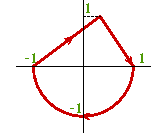
\includegraphics{05clockwise-contour-problem.pdf}
\end{center}
In this drawing the circle has radius $1$, and the height of the triangle is
also $1$.  The orientation of the curve is in the direction of the arrows.

\problem  Let  $\cR$ be the unit square, i.e.~$\cR=\{(x,y) : 0\le x,y\le 1\}$.
Let $\cC$ be the boundary of the square $\cR$ traversed in counterclockwise sense.

\subprob Compute $\DS\int_\cC 2y\,dx + 3x\,dy$ by finding parametrizations of
the edges and applying the definition of the line integral.

\subprob Compute $\DS\int_\cC 2y\,dx + 3x\,dy$ by applying Green's theorem and
computing a suitable double integral over $\cR$.
\answer
The answer in both cases is the same (because they are two different ways of
computing the same integral).  The second approach, using Green's theorem leads to
\[
\int_\cC 2y\,dx + 3x\,dy
= \iint\limits_\cR \Bigl(\pdd{3x}x - \pdd{2y}y\Bigr)dA
= \iint\limits_\cR (3-2)\,dA,
\]
so the answer is the area of the square, i.e.~$1$
\endanswer

\problem Compute $\DS\oint_{\cC} \nab(x^2y^2)\dpp\vT\, ds$ where $\cC$ is the counter
clockwise traversed boundary of the region $\cR$ defined by $x^2+y^2<16$.
\answer
Using Green's theorem we get zero.  But here we do not need Green's theorem: the
Fundamental Theorem for line integrals (see
\S~{sec:integral-over-closed-curve-of-gradient-vanishes}) tells us that this integral must be zero.
\endanswer

\problem A gas is flowing in the plane with velocity field 
\[
\vv(x, y) =
\vek 1 \\ -y\tor.
\]  

\subprob Draw the vector field.

\subprob How much gas flows out of the rectangle $\cR$ defined by $0<x<L$, $-H<y<H$?
\end{multicols}
\problem In each of the following problems $\cC$ is the counter clockwise
traversed boundary of the region $\cD$ and you are asked to compute the
indicated line integral in two ways: directly, and by using Green's Theorem.

\begin{tabbing}
\=\hspace{0.5\textwidth}\=\kill
\>\subprob  $\DS\oint_\cC  xy\,dx + xy\,dy$, 
\>$\cR:0\le x,y\le 1$.
\answer $0$
\endanswer
\\[1ex]
\>\subprob  $\DS\oint_\cC  e^{2x+3y}\,dx + e^{xy}\,dy$, 
\> $\cR:-2\le x\le 2$, $-1\le y\le 1$.
\answer $1/(2e)-1/(2e^7)+e/2-e^7/2$
\endanswer
\\[1ex]
\>\subprob  $\DS\oint_\cC \vF\dpp\vT ds$,\quad $\vF(x, y) = \tvek y\cos x\\  y\sin
x\ttor$, 
\> $\cR:0\le x\le \pi/2$, $1\le y\le 2$.
\answer $1/2$
\endanswer
\\[1ex]
\>\subprob  $\DS\oint_\cC  xy^2\,dx + x^2y\,dy$, 
\> $\cR:0\le x\le 1$, $0\le y\le x$.
\answer
$0$
\endanswer
\\[1ex]
\>\subprob  $\DS\oint_\cC  x^2y\,dx + xy^2\,dy$, 
\> $\cR:0\le x\le 1$, $0\le y\le x$.
\answer $-1/6$
\endanswer
\\[1ex]
\>\subprob  $\DS\oint_\cC  x\sqrt{y}\,dx + \sqrt{x+y}\,dy$, 
\> $\cR:1\le x\le 2$, $2x\le y\le 4$.
\answer $(2\sqrt3-10\sqrt5+8\sqrt6)/3-2\sqrt2/5+1/5$
\endanswer
\\[1ex]
\>\subprob  $\DS\oint_\cC  (x/y)\,dx + (2+3x)\,dy$, 
\> $\cR:1\le x\le 2$, $1\le y\le x^2$.
\answer $11/2-\ln(2)$
\endanswer
\\[1ex]
\>\subprob  $\DS\oint_\cC  \sin y\,dx + \sin x\,dy$, 
\> $\cR:0\le x\le \pi/2$, $x\le y\le \pi/2$.
\answer $2-\pi/2$
\endanswer
\\[1ex]
\>\subprob  $\DS\oint_\cC  x\ln y\,dx$,
\> $\cR:1\le x\le 2$, $\DS e^x\le y\le e^{x^2}$.
\answer $-17/12$
\endanswer
\\[1ex]
\>\subprob  $\DS\oint_\cC  \sqrt{1+x^2}\,dy$, 
\> $\cR:-1\le x\le 1$, $x^2\le y\le 1$.
\answer $0$
\endanswer
\\[1ex]
\>\subprob  $\DS\oint_\cC  x^2y\,dx - xy^2\,dy$, 
\> $\cR:x^2+y^2\le 1$.
\answer $-\pi/2$
\endanswer
\\[1ex]
\>\subprob  $\DS\oint_\cC \vv\dpp\vN\, ds$,\quad $ \vv(x,y) = \tvek xy^2\\x^2y\ttor$, 
\> $\cR:x^2+y^2\le 1$,\quad $\vN$ the outward normal.
\answer $-\pi/2$
\endanswer
\\[1ex]
\>\subprob  $\DS\oint_\cC  y^3\,dx + 2x^3\,dy$, 
\> $\cR:x^2+y^2\le 4$.
\answer $12\pi$
\endanswer

\end{tabbing}

\noproblemfont

\section{Surfaces and Surface integrals}
\label{sec:surfaces}
In addition to integrals over two and three dimensional domains, and line
integrals over curves in the plane or in space, one can also integrate over
surfaces.  In this section we will give a quick introduction to surfaces and
surface integrals.  For an in-depth study of the subject, students should
consider taking a more advanced course on vector calculus, such as Math~321.
\begin{figure}[h]
  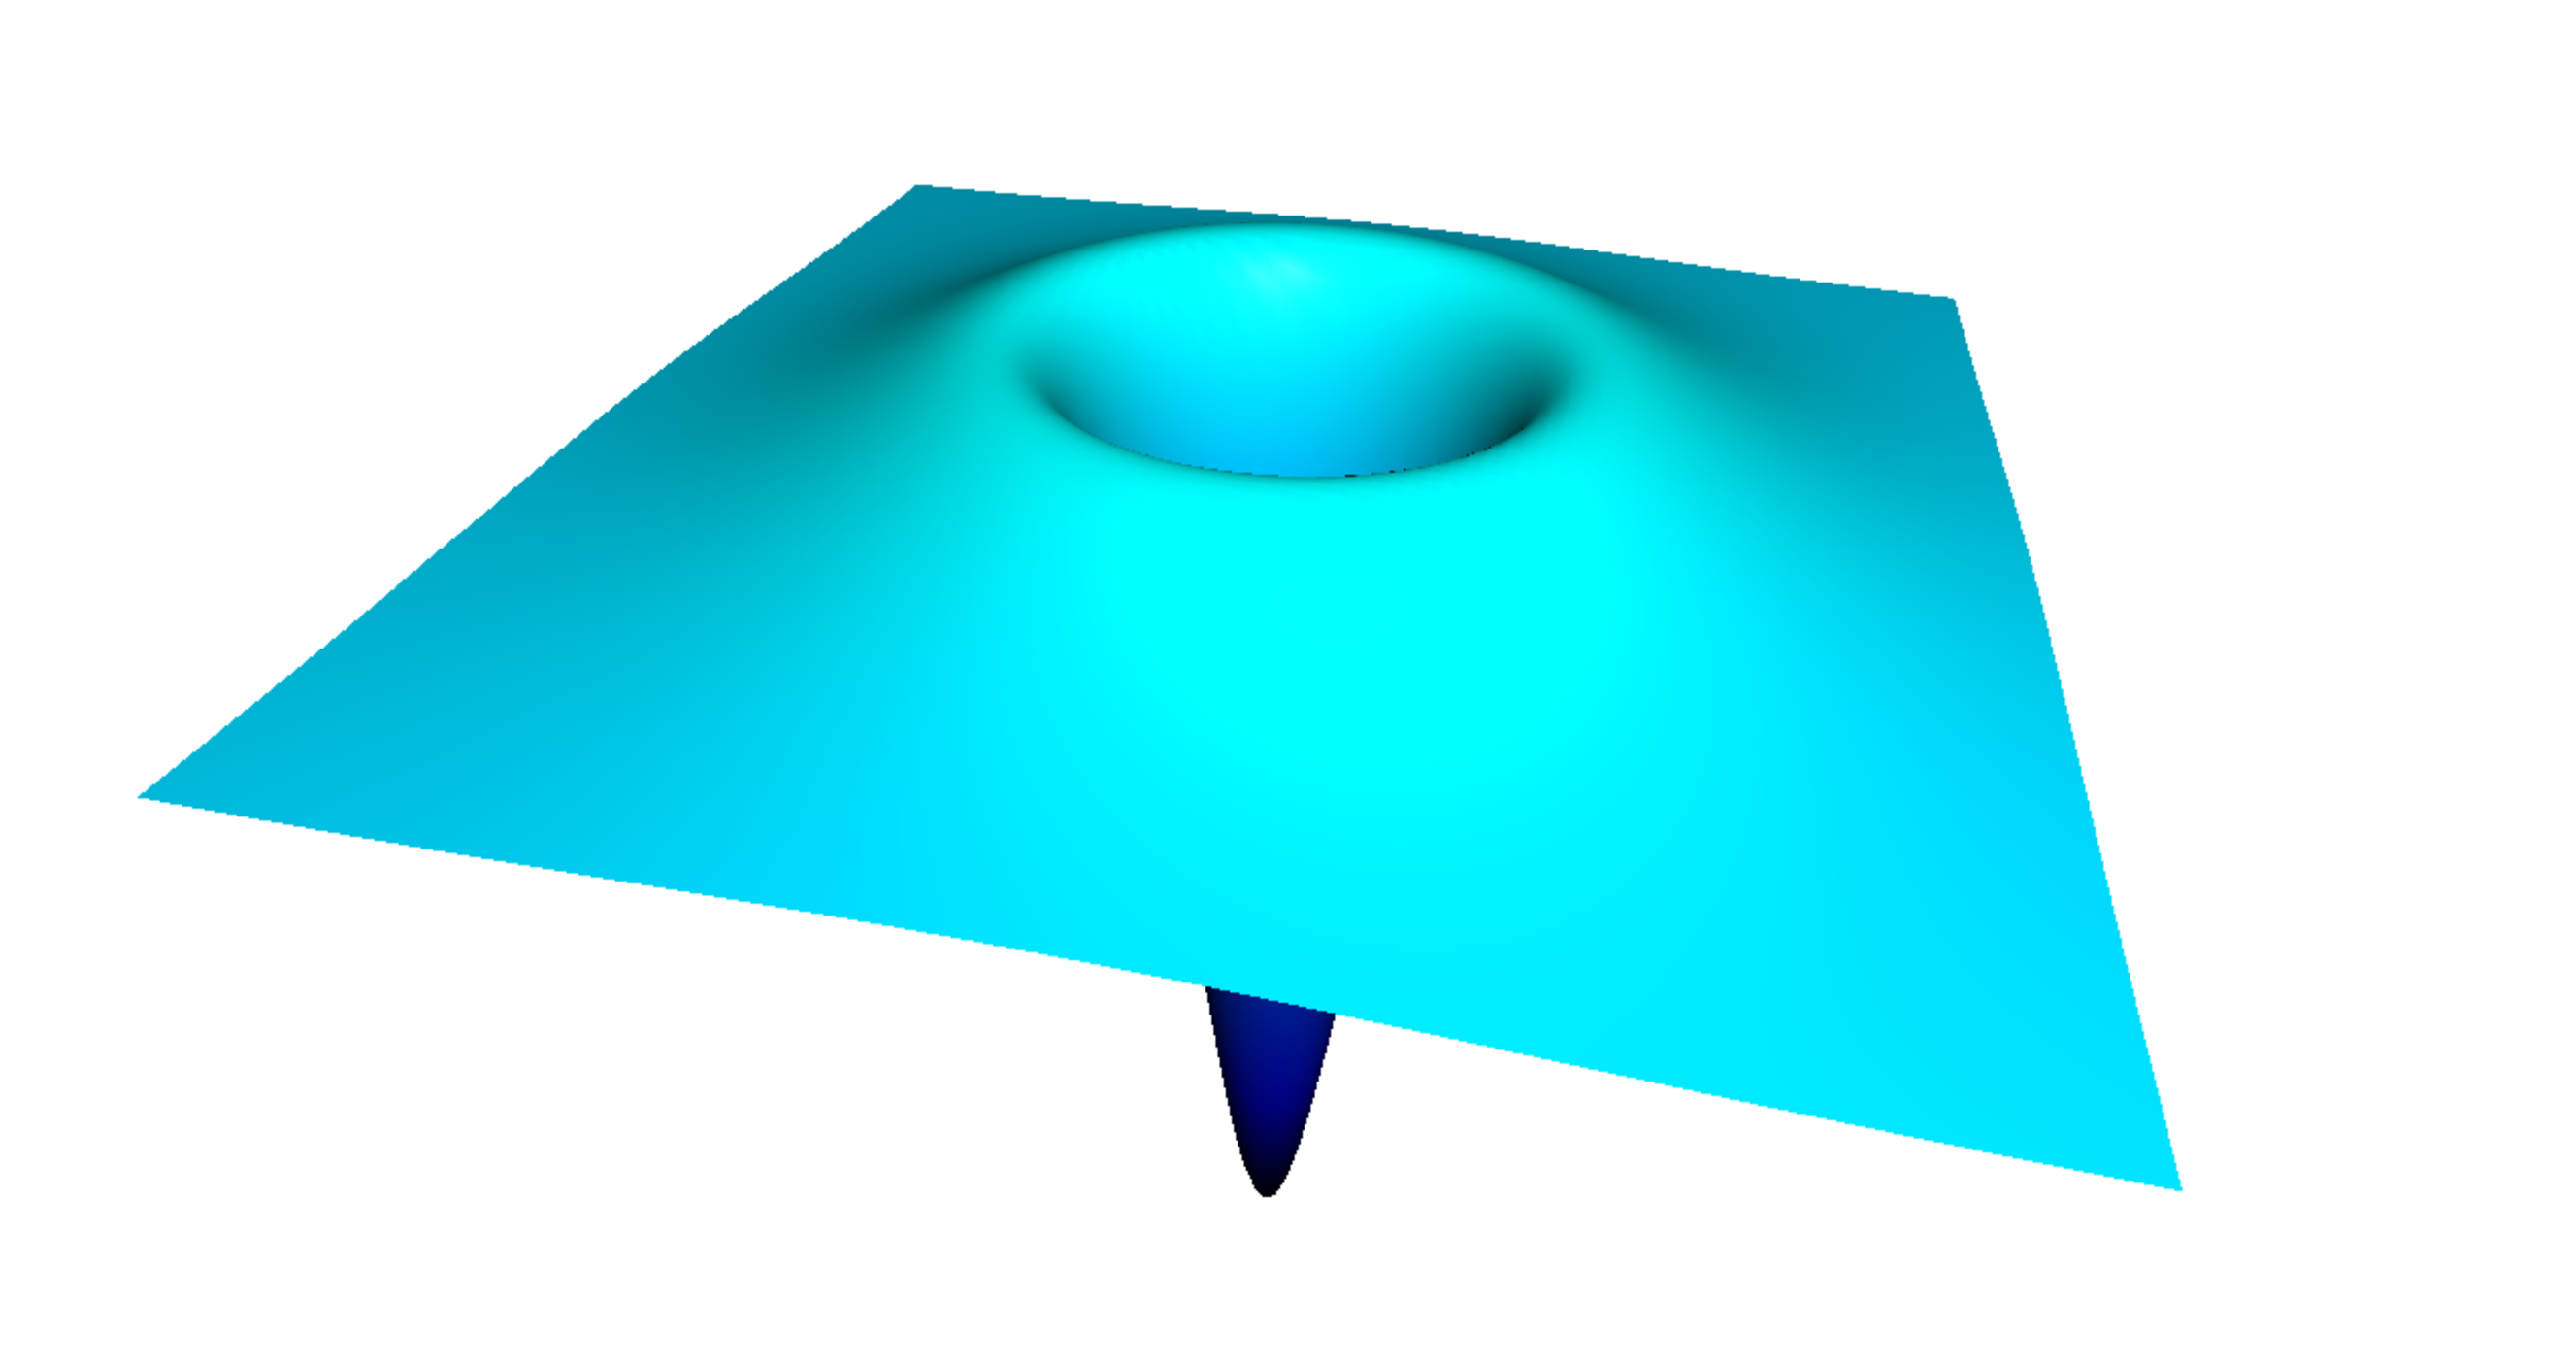
\includegraphics[width=0.3\textwidth]{05bump.pdf}
  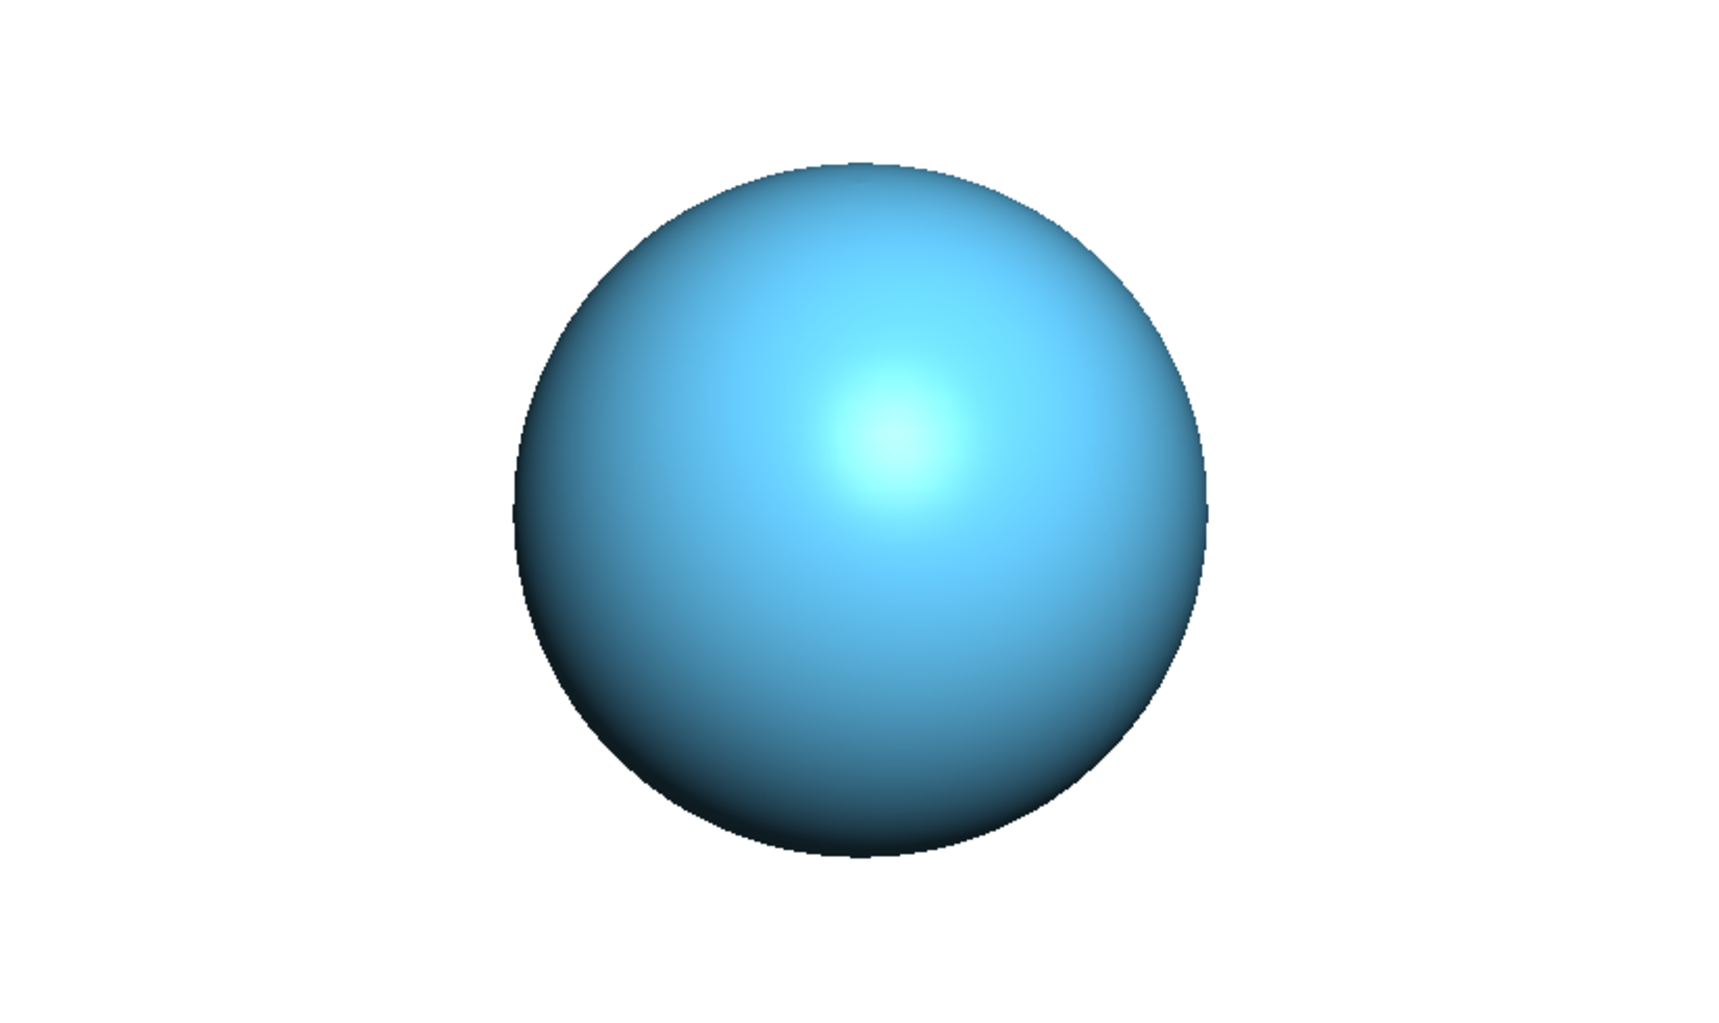
\includegraphics[width=0.3\textwidth]{05sphere-shiny.pdf}
  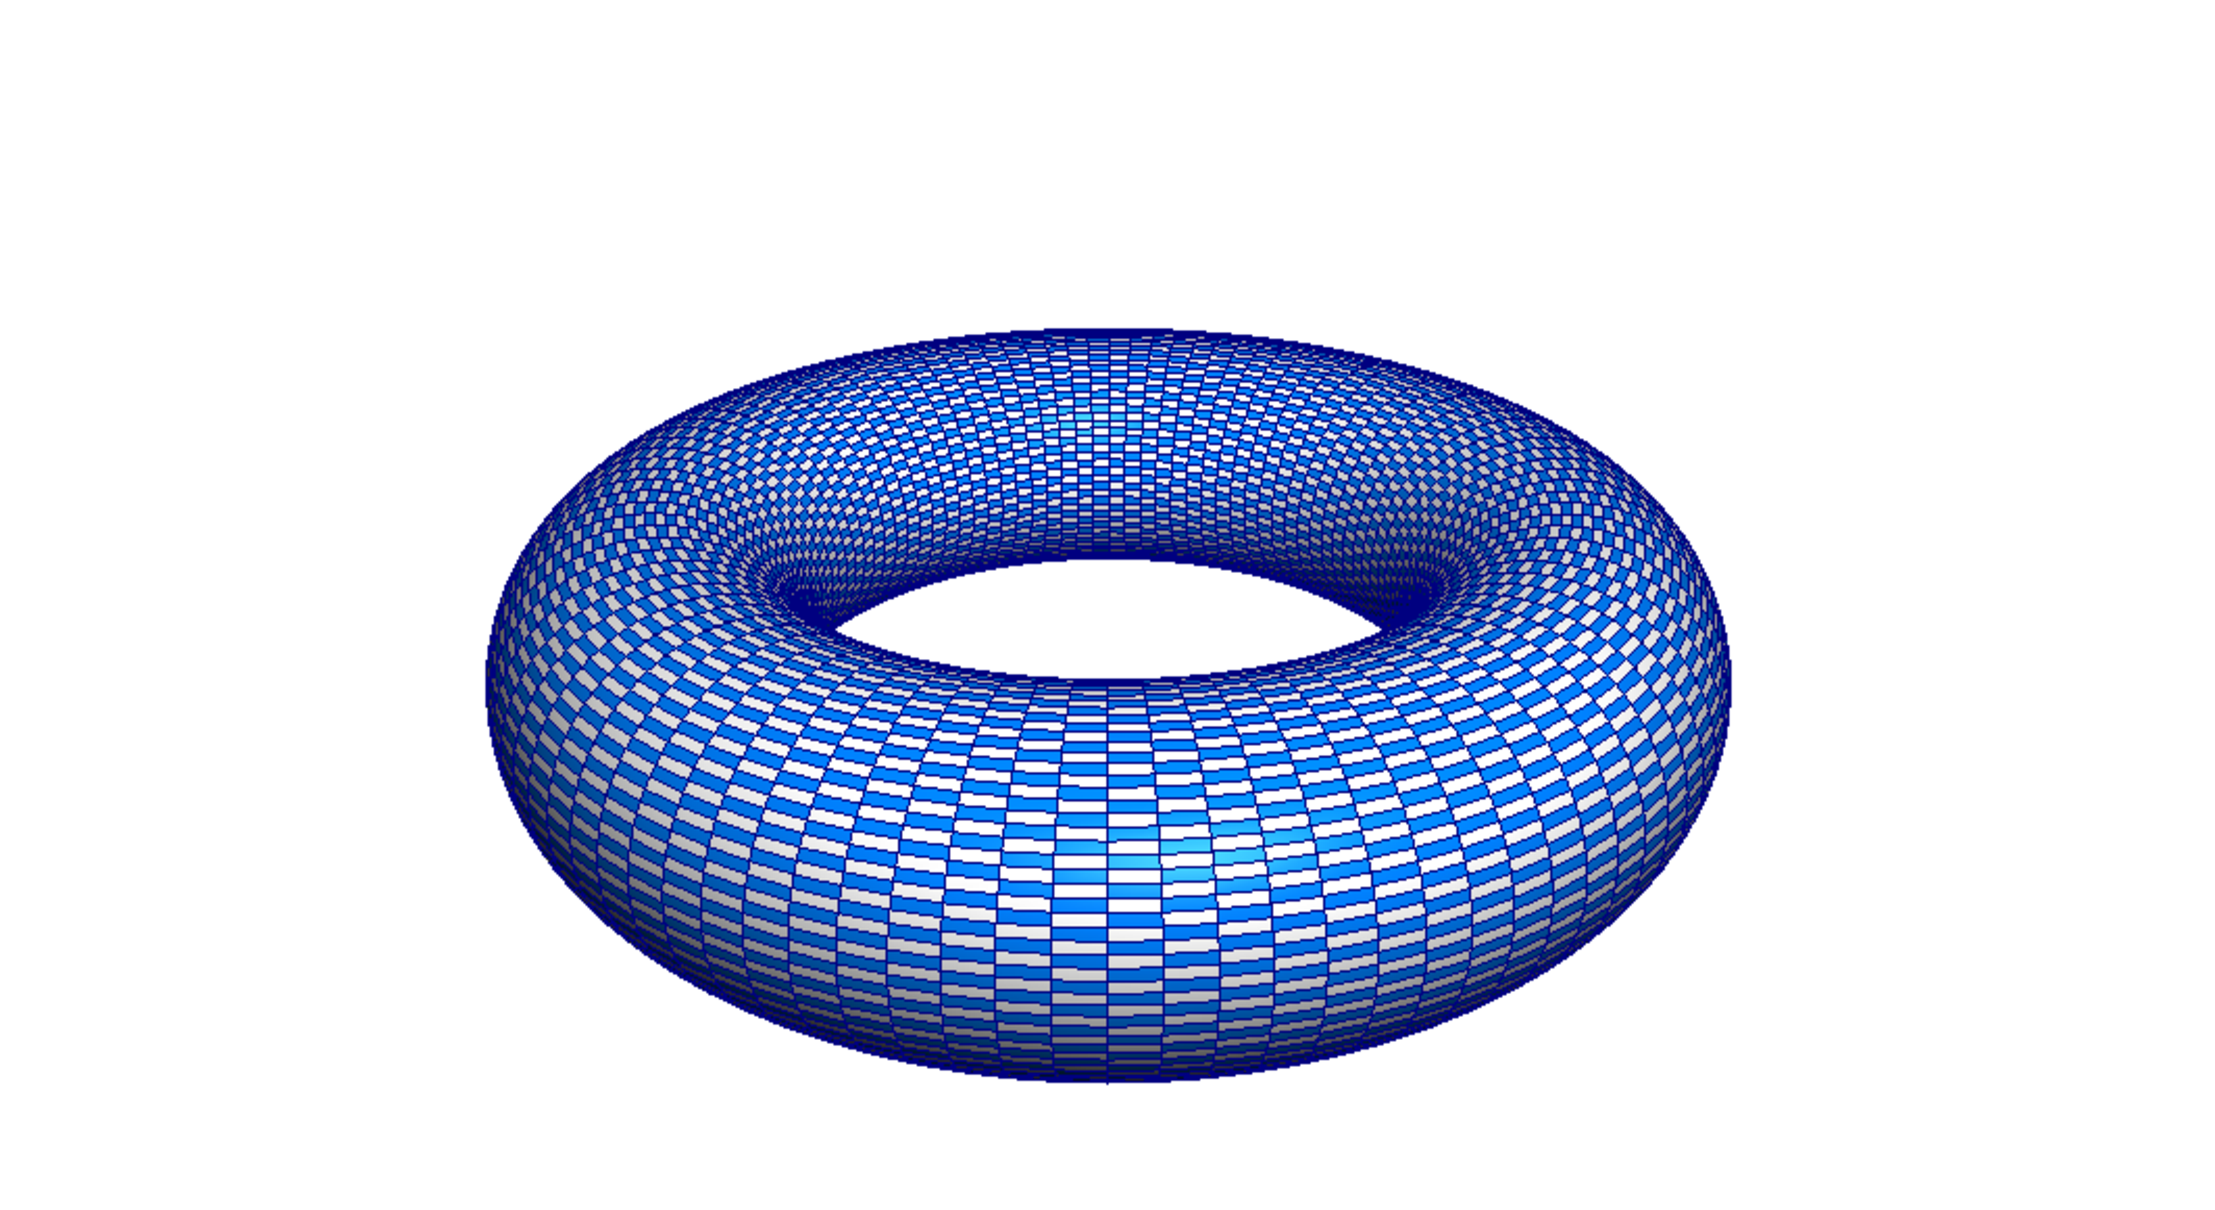
\includegraphics[width=0.3\textwidth]{05torus.pdf}
  \caption{Two dimensional surfaces.}
\end{figure}

\subsection{Surfaces and surface patches}
\label{sec:surface-patches}
We can think of a curve as the result of taking a line and bending it into some
curved shape.  In the same way a surface can be thought of as the result of
taking a portion of a flat plane and bending and twisting it into some other
shape.
Just as some curves appear as the boundaries (or edges) of plane domains, some
surfaces appear as boundaries of domains in three dimensional space.  For
example, the sphere centered at the origin and with radius $R$
\begin{equation}
  x^2+y^2+z^2 = R^2
  \label{eq:sphere-defining-equation}
\end{equation}
is the boundary of the three dimensional ball it encloses.

Surfaces can be described using ``defining equations,'' i.e.~by specifying an
equation whose zero set is the intended surface.  For example, the sphere of
radius $R$ has \eqref{eq:sphere-defining-equation} as defining equation.  For
purposes of integration it is more convenient to represent surfaces in terms of
\emph{surface patches.}  These are the surface analog of parametrized curves.
\medskip

\subsubsection*{Definition}\itshape A surface patch is a differentiable vector
\label{sec:surface-patch-definition}
function of two variables\upshape
\[
\vx = \vx(u,v), \qquad a\leq u\leq b,\quad c\leq v\leq d.
\]

\begin{figure}\def\svgwidth{360pt}
  %\input ../figures/234/05normal-and-surface-element.pdf_tex
  \input ../figures/234/05patch-lines-of-constant-u-v.pdf_tex
  \caption{\textbf{A surface patch.}  A vector function $\vx$ of two variables
  $u$ and $v$ maps a piece of the $uv$-plane into three dimensional space.  The
  rectangular grid in the $uv$ domain gets mapped onto a network of curves on the
  surface patch $\cS$.  If the rectangular grid in the $uv$-domain is sufficiently
  fine, then the corresponding curves on the surface divide the surface patch into
  small pieces that are approximately parallelograms.  }
  %\label{fig:normal-and-surface-element}
  \label{fig:patch-and-lines-of-constant-u-v}
\end{figure}


\begin{figure}[t]
  \input ../figures/234/05graph-patch.pdf_tex
  \caption{\textbf{A graph as a surface patch: } the graph of a function $z=f(x,y)$ can be represented as a surface patch.  The vector function $\vx	$ that parametrizes the graph is $\vx(u,v) = u\ves1+v\ves2+f(u,v)\ves3$.}
  \label{fig:graph-as-surface-patch}
\end{figure}
\subsection{Example -- the graph of a function is a surface patch}
\label{sec:graph-is-patch}
If $z=f(x, y)$ is a function defined for $a\leq x\leq b$, $c\leq y\leq d$, then its
graph can be thought of as a surface patch, where
\begin{equation}
  \vx(u,v) = \vek u \\ v \\ f(u,v) \tor.
  \label{eq:graph-patch}
\end{equation}
In words: we take the $x$ and $y$ coordinates as parameters, setting $x=u$ and $y=v$.
The $z$ component of any point on the patch is then $z=f(x,y) = f(u,v)$.

\subsection{Example -- the sphere as a surface patch}
The sphere is a two dimensional surface, and one way to parametrize it is to use
spherical coordinates.  Thus 
\begin{equation}
  \vx(\theta, \varphi) = \vek
  R \cos\varphi \sin\theta\\
  R \sin\varphi \sin\theta\\
  R \cos \theta
  \tor
  \label{eq:sphere-patch}
\end{equation}
with
\[
  0\leq \theta\leq\pi, \quad 0\leq\varphi\leq 2\pi
\]
is a surface patch that parametrizes the sphere: it is a parametrization of the sphere.
See \S VI-\ref{sec:spherical-coordinates} where spherical coordinates were defined,
and see Figure~\ref{fig:sphere-patch} for a picture.

All points with $\theta=0$ are mapped to the ``north pole''; all points with
$\theta=\pi$ correspond to the ``south pole''; the points with $\theta=\frac12\pi$
form the ``equator.''

\begin{figure}[h]
  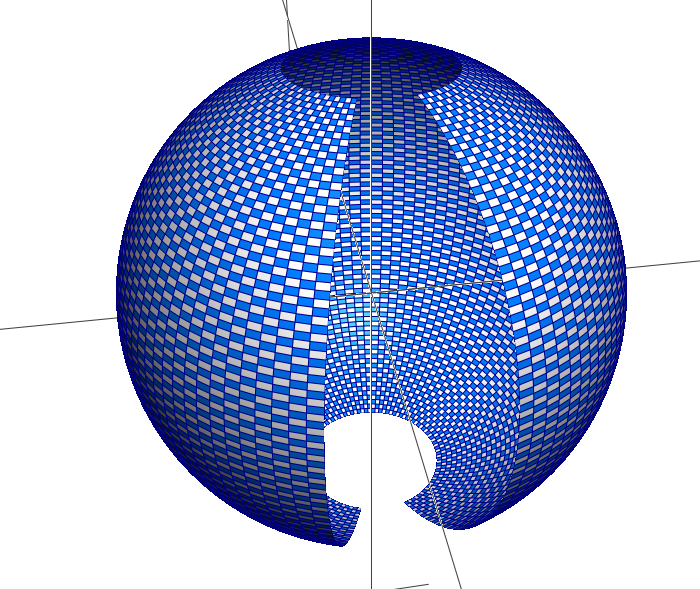
\includegraphics[width=0.5\textwidth]{05sphere-patch.png}
  \caption{\textbf{Sphere: } a piece of the sphere parametrized by the surface patch in
  \eqref{eq:sphere-patch}.  Shown is the piece with $0.1\pi\leq \theta \leq 0.9\pi$
  and $0.1\pi\leq \varphi \leq 1.9\pi$.  }
  \label{fig:sphere-patch}
\end{figure}

\subsection{Area of a surface patch}
\label{sec:area-and-normal-for-patch}
For any given surface we can ask ``what is its surface area?''  The intuitive
interpretation of this could be
\begin{equation}
  \textit{\dfnt ``how much paint do we need to cover one side of the surface?'' }
  \label{eq:how-much-paint-do-we-need}
\end{equation}
or
\begin{equation}
  \textit{\dfnt ``how much paper to we need to make the surface?''}
  \label{eq:how-much-paper}
\end{equation}
Neither interpretation stands up to closer scrutiny:  there are surfaces, like
the M\"obius strip in Figure~\ref{fig:mobius}, that only have one side, so that
\begin{figure}[h]
  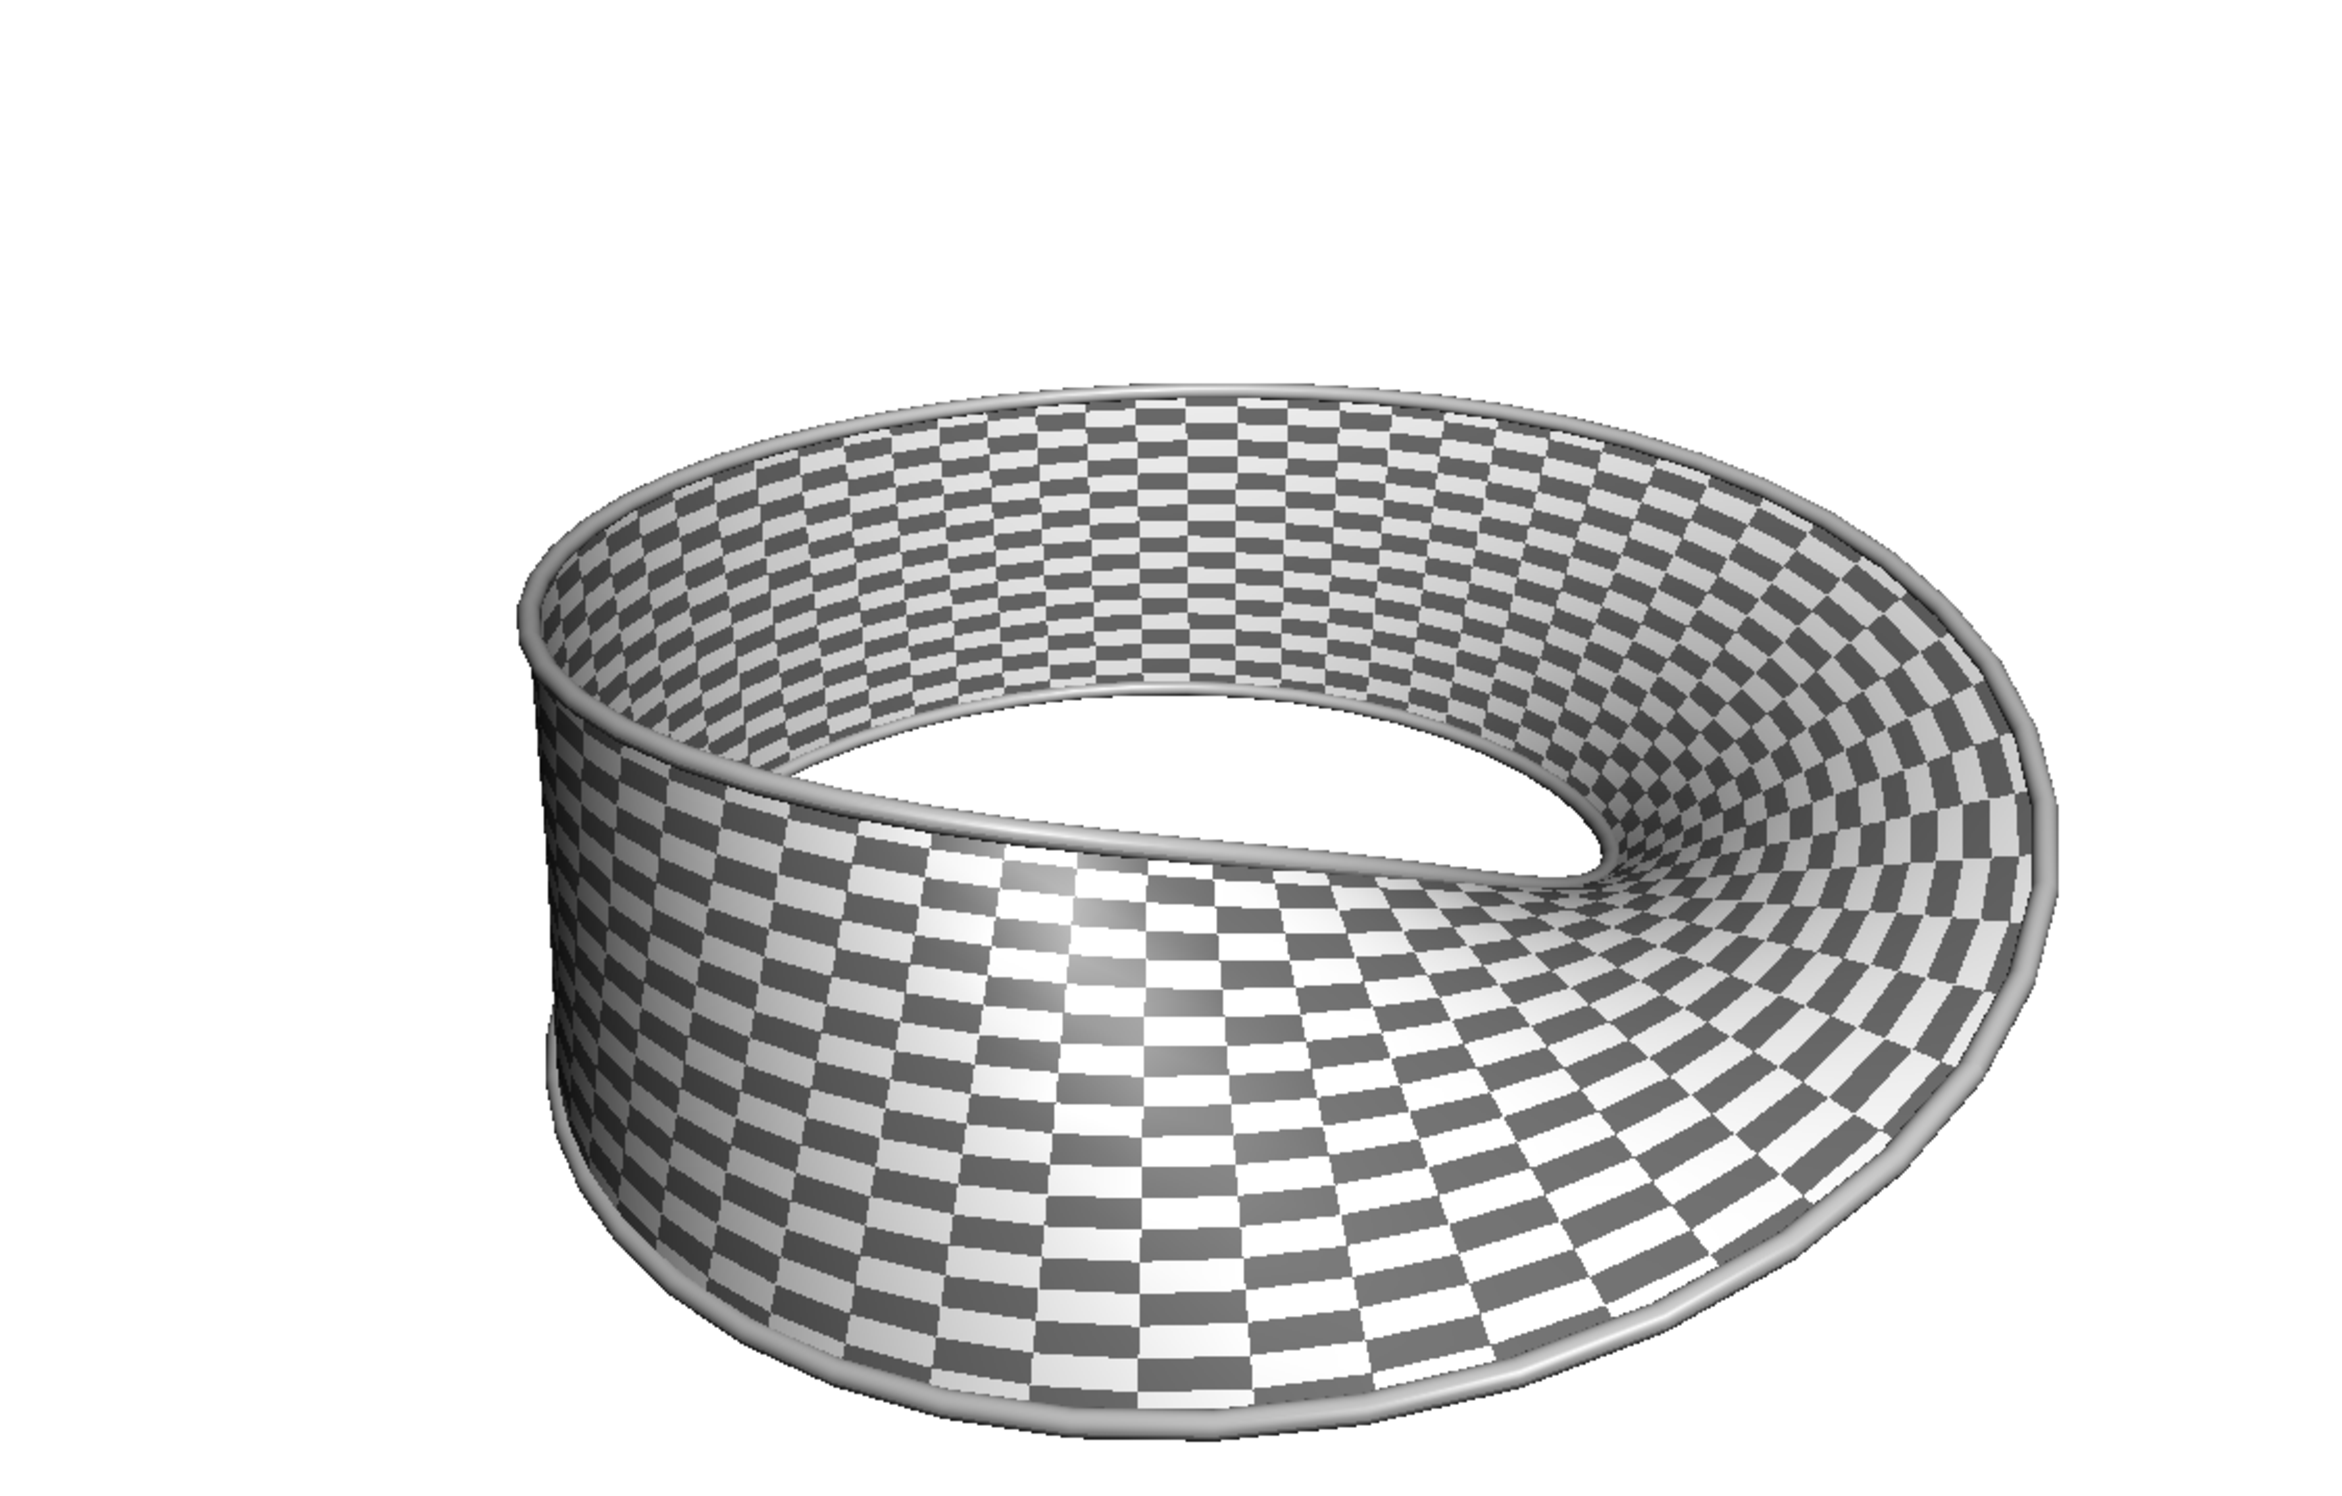
\includegraphics[width=2in]{Mobius_with_patches.pdf}
  \caption{\textbf{A M\"obius strip.}  What is the surface area of this strip, and
  how many square inches of paper do we need to make one?}
  \label{fig:mobius}
\end{figure}
questions~\eqref{eq:how-much-paint-do-we-need} and~\eqref{eq:how-much-paper} will give
different answers.  On the other hand, while it is possible to take a flat piece of
paper and bend it in the shape of a cylinder, a cone, or a M\"obius strip, it is not
possible to bend a flat piece of paper into a sphere without ripping or stretching it
(and thus changing its area.)

In spite of these (and other) issues we will argue from intuition and derive a
formula for the area of a surface patch.  The story is very similar to the derivation
of the arc length of a parametrized curve in \S~II.\ref{sec:arc-length}.

\begin{figure}[h]\def\svgwidth{360pt}
  \input ../figures/234/05normal-and-surface-element.pdf_tex
  \caption{Computing the area and normal to a surface patch.  The small rectangle in
  the $uv$-domain gets mapped to a small region on the surface patch.  This small
  region is almost a parallelogram whose sides are given by the vectors $\vx_u \Delta
  u$ and $\vx_v\Delta v$.}
  \label{fig:normal-and-surface-element}
\end{figure}

If $\vx(u,v)$ is a surface patch with domain $a\leq u\leq b$, $c\leq v\leq d$, then
we divide its domain into many small rectangular pieces of size $\Delta u$ by $\Delta
v$ by partitioning both the $u$ and $v$ intervals. See the left half of
Figure~\ref{fig:normal-and-surface-element}.  This leads to a partitioning of the
surface patch into small regions, each of which is approximately a parallelogram (on
the right in Figure~\ref{fig:normal-and-surface-element}).  We compute the area of
the surface patch by adding the areas of all these smaller pieces.  Since any such
piece is approximately a parallelogram, we can find its area by computing the cross
product of the vectors defined by its edges.
\begin{figure}[h]
  \input ../figures/234/05area-element.pdf_tex
  \caption{The small blue rectangle in the $uv$-plane from
  Figure~\ref{fig:normal-and-surface-element}, and its image on the surface patch.}
  \label{fig:small-area-element}
\end{figure}
To find these edges consider Figure~\ref{fig:small-area-element}.  In a small
partition piece on the surface patch, the parameter $u$ is allowed to vary between
some value $u_0$ and $u_0+\Delta u$, while the other parameter $v$ is allowed to vary
between some $v_0$ and $v_0+\Delta v$.  One edge of the surface patch (on the right
in Figure~\ref{fig:small-area-element}) represents the change in $\vx(u, v)$
as $u$ is increased by $\Delta u$, while keeping $v$ constant; i.e.~ it is
\[
  \vx(u_0+\Delta u, v_0) - \vx(u_0, v_0) \approx \pdd{\vx}u (u_0, v_0) \cdot \Delta u.
\]
The other edge represents the change in $\vx(u, v)$ when $v$ is increased by $\Delta
v$ and is thus given by
\[
  \vx(u_0, v_0+\Delta v) - \vx(u_0, v_0) \approx \pdd{\vx}v (u_0, v_0) \cdot \Delta v.
\]
The area of the small parallelogram on the surface patch is therefore the length of
the cross-product of these two vectors:
\begin{align*}
  \Delta A &\approx \left\| \pdd{\vx}u (u_0, v_0) \cdot \Delta u
  \; \cp \; 
  \pdd{\vx}v (u_0, v_0) \cdot \Delta v
  \right\|\\[3pt]
  &= \|\vx_u\cp\vx_v\| \, \Delta u\, \Delta v.
\end{align*}
Adding this over all pieces that make up the surface patch gives us the total area of
the patch:
\begin{equation}
  \textsf{Area of $\cS$} = \int_c^d \int_a^b \|\vx_u\cp\vx_v\| \,du\,dv .
  \label{eq:area-of-surface-patch}
\end{equation}
The quantity that appears in this integral appears in many other surface integrals
and is called ``the area element'' of the surface patch $\vx$.  The usual notation
for this quantity is
\begin{equation}
  dA = \|\vx_u\cp\vx_v\| \,du\,dv,
  \label{eq:area-element-for-surface-patch}
\end{equation}
and it is thought of as the ``area of an infinitesimally small piece of the
surface.''  

\subsection{Surface integrals}
\label{sec:surface-integrals}
If $f(x, y, z)$ is some function that is defined on the surface (e.g.~a density of
some kind), then one defines its integral over the surface to be
\begin{equation}
  \liint_{\cS} f(x, y, z)\, dA
  =
 \int_c^d \int_a^b f(\vx(u,v))\,\|\vx_u\cp\vx_v\| \,du\,dv .
  \label{eq:surface-integral-def}
\end{equation}
Here $f(\vx(u,v))$ is the result of substituting the surface parametrization
$\vx(u,v)$ in the function.

\subsection{Unit normal to a surface patch}
\label{sec:unit-normal-to-patch}
From Figures~\ref{fig:normal-and-surface-element} and~\ref{fig:small-area-element} it
appears that both vectors $\vx_u$ and $\vx_v$ are tangent to the surface, and that
their cross product $\vx_u\cp\vx_v$ is perpendicular to the surface.  We adopt this
as the definition of the tangent plane and normal direction to the surface:
\medskip

\subsubsection*{Definition}\itshape Let $\vx$ be a surface patch, and let $X_0$ be a
point with position vector $\vx(u_0,v_0)$ on the surface patch.  If
\[
  \vm \stackrel{\text{\dfnt def}}=\vx_u(u_0,v_0) \cp \vx_v(u_0,v_0)\neq \vvv0,
\]
then the vector $\vm$ defines the normal direction to the surface. The tangent
plane to the surface through $X_0$ is the plane with normal vector $\vm$ that goes
through $X_0$.\upshape\medskip

In general the vector $\vm$ does not have unit length, and one often needs a normal
vector with length one for the surface.  Thus one defines
\begin{equation}
  \vN = \frac{\vm}{\|\vm\|} = \frac{\vx_u\cp\vx_v}{\|\vx_u\cp\vx_v\|}
  \label{eq:unit-normal-to-patch}
\end{equation}
to be the \emph{unit normal} for the surface patch $\vx$.  Note that $-\vN$ also is a unit vector that is normal to the surface.  

\subsection{Flux across a surface patch}
\label{sec:flux-across-a-surface-patch}
In \S~\ref{sec:flux-integrals} we defined the flux across a curve of
a vector field $\vv$ (which we think of as the velocity field of some flowing
liquid or gas).  The set-up in \S~\ref{sec:flux-integrals} was
purely two dimensional.  Now that we have introduced surface integrals we can
formulate the same concept for the more realistic situation of a fluid flowing
through three dimensional space with velocity field $\vv$.  We define the
\emph{flux of a vector field $\vv$ across a surface patch} to be
\begin{equation}
  \textsf{Flux}
  = \liint_{\cS} \vv\dpp\vN\, dA
  \label{eq:flux-through-surface-patch}
\end{equation}
We have expressions for both $\vN$ and $dA$ (namely,
\eqref{eq:area-element-for-surface-patch} and \eqref{eq:unit-normal-to-patch}).
When put together, they simplify to
\[
  \vN\, dA = \frac{\vx_u\cp\vx_v}{\|\vx_u\cp\vx_v\|}\cdot\|\vx_u\cp\vx_v\|\, du\,dv 
  = \vx_u\cp\vx_v \, du\,dv 
\]
Therefore the flux integral can be computed as
\begin{equation}
\liint_{\cS} \vv\dpp\vN\, dA
= \int_c^d\int_a^b \vv\dpp(\vx_u \cp \vx_v)\, du\,dv.
  \label{eq:flux-through-patch}
\end{equation}

\section{Examples}
\label{sec:examples-of-surface-integrals}
\subsection{Area and unit normal of a sphere}
\label{sec:area-of-sphere-example}
The sphere with radius $R$ can be represented by the surface patch
\begin{equation}
  \vx(\theta,\varphi) = 
  \vek 
  R\cos\varphi \sin\theta \\
  R\sin\varphi \sin\theta \\
  R\cos\theta
  \tor,
  \label{eq:sphere-patch-example}
\end{equation}
for which we have
\[
  \vx_\theta = R \vek
  \cos\varphi \cos\theta \\
  \sin\varphi \cos\theta \\
  -\sin\theta
  \tor,
  \qquad
  \vx_\varphi = R \vek
  -\sin\varphi \sin\theta \\
  \cos\varphi \sin\theta \\
  0
  \tor
\]
and hence
\begin{align*}
  \vx_\theta\cp\vx_\varphi
  &= R^2
  \vek
  \cos\varphi \sin^2\theta \\
  \sin\varphi \sin^2\theta \\
  \cos^2\varphi \sin\theta\cos\theta +
  \sin^2\varphi \sin\theta\cos\theta 
  \tor \\
  &= R^2
  \vek
  \cos\varphi \sin^2\theta \\
  \sin\varphi \sin^2\theta \\
  \sin\theta\cos\theta 
  \tor \\
  &=R^2\sin\theta \vek
  \cos\varphi \sin\theta \\
  \sin\varphi \sin\theta \\
  \cos \theta
  \tor.
  \label{eq:xtheta-cross-xphi-sphere}
\end{align*}
The length of $\vx_\theta\cp\vx_\varphi$ is
\[
  \|\vx_\theta\cp\vx_\varphi\|
  =R^2\sin\theta\;  \left\|\vek
  \cos\varphi \sin\theta \\
  \sin\varphi \sin\theta \\
  \cos \theta
  \tor
  \right\| 
  =R^2\sin\theta.
\]
and the area element on the sphere is
\[
  dA = R^2\sin\theta \, d\theta\,d\varphi.
\]
Integrating over the sphere gives us the area of the sphere:
\begin{equation}
  \textsf{Area of sphere}
  =
  \int_{\varphi=0}^{2\pi} \int_{\theta=0}^\pi
  R^2 \sin \theta\, d\theta\, d\varphi
  =
  4\pi R^2,
  \label{eq:area-of-sphere-example}
\end{equation}
which is the familiar answer.

We also find from our formula for $\vx_\theta\cp\vx_\varphi$
that the unit normal at the point with position vector $\vx(\theta,
\varphi)$ is
\[
  \vN = \frac{\vx_\theta\cp\vx_\varphi}{\|\vx_\theta\cp\vx_\varphi\|}
  = \vek
  \cos\varphi \sin\theta \\
  \sin\varphi \sin\theta \\
  \cos \theta
  \tor
\]%
\begin{figure}[h]
  \input ../figures/234/05sphere-unit-normal.pdf_tex
  \caption{The unit normal at a point on a sphere centered at the origin has the same
  direction as the position vector of the point.}
  \label{fig:sphere-unit-normal}
\end{figure}

Looking back at the definition~\eqref{eq:sphere-patch-example} of our surface patch
we see that 
\[
  \vx = R\vN, \text{ or, } \vN = \frac{\vx}{R}.
\]
In words: the unit normal is just the position vector $\vx$ rescaled to length one.
Perhaps with hindsight, this should be clear from a drawing of the sphere
(e.g.~Figure~\ref{fig:sphere-unit-normal}).  In many geometrically simple situations
it is often easier to guess the unit normal from a drawing than by going through a
computation like the one we did in this example.  And sometimes it is even possible to compute the area element without working out $\vx_u$, $\vx_v$, and their cross product.  For instance, it is possible to derive our formula for the area element $dA = R^2 \sin\theta d\theta d\varphi$ from a drawing like Figure~VI.\ref{fig:04spherical-volume-element}.
 

\subsection{The flux of a vector field across the sphere}
\label{sec:flux-across-sphere}
We consider the velocity field of the expanding gas from
\S~\ref{sec:expanding-flow-example} again, except we now consider a gas occupying
three dimensional space:
\[
  \vv = \frac{V_0}{R_0} \vx.
\]
Here $V_0$ and $R_0$ are constants: $V_0$ is the velocity of the gas when it has
reached distance $R_0$ from the origin.

We compute the flux
\[
  \text{\dfnt Flux} = \liint_{\cS_R} \vv\dpp\vN\, dA
\]
of this velocity field across the sphere $\cS_R$ with radius $R$ in two ways.

First, we use the formula for $\vN\, dA$ 
\[
  \vN\,dA = \vx_\theta\cp\vx_\varphi \,d\varphi\,d\theta
  = R^2\sin\theta
  \vek
    \cos\varphi \sin\theta \\
    \sin\varphi \sin\theta \\
    \cos \theta
  \tor \,d\varphi\,d\theta
\]
and compute
\begin{align*}
  \text{\dfnt Flux}
  &= 
  \int_{\theta=0}^\pi \int_{\varphi=0}^{2\pi}
  \frac{V_0}{R_0} \vx \dpp R^2\sin\theta
  \vek
  \cos\varphi \sin\theta \\
  \sin\varphi \sin\theta \\
  \cos \theta
  \tor \,d\varphi\,d\theta \\
  &=\frac{V_0}{R_0}R^2 \int_{\theta=0}^\pi \int_{\varphi=0}^{2\pi}
   \vek
  R\cos\varphi \sin\theta \\
  R\sin\varphi \sin\theta \\
  R\cos \theta
  \tor\dpp   \vek
  \cos\varphi \sin\theta \\
  \sin\varphi \sin\theta \\
  \cos \theta
  \tor \sin\theta \,d\varphi\,d\theta \\
  &=
  \frac{V_0}{R_0}R^3 \int_{\theta=0}^\pi \int_{\varphi=0}^{2\pi} 
  \sin\theta \,d\varphi\,d\theta \\
  &= 4\pi\frac{V_0}{R_0}R^3.
\end{align*}

The second approach is more geometrical and avoids computing any integrals.  We begin
by noting that the unit normal on the sphere at the point with position vector $\vx$
is $\vN = \vx/R$, and hence that 
\[
  \vv\dpp\vN
  = \frac{V_0}{R_0} \vx\dpp\frac{\vx}{R} 
  = \frac{V_0}{R_0} \frac{\vx\dpp\vx}{R} 
  = \frac{V_0}{R_0} \frac{R^2}{R} 
  = V_0 \frac{R}{R_0}.
\]
The quantity we want to integrate is therefore constant.  We find that the flux is 
\[
  \text{\dfnt Flux} = \liint_{\cS} V_0 \frac{R}{R_0} dA
  = V_0 \frac{R}{R_0}\cdot\text{\dfnt Area of $\cS$}
  = V_0 \frac{R}{R_0} \cdot 4\pi R^2,
\]
which is the same as we got using the first approach.

\section{The divergence theorem and Stokes' theorem}
\label{sec:divergence-and-stokes}

\subsection{The divergence theorem in three dimensions}
\label{sec:divergence-three-dim}\itshape
If $\cS$ is a surface that encloses a three dimensional region $\cR$, if $\vv$
is a vector field that is defined and differentiable on all of $\cR$, and if
$\vN$ is the outward unit normal on $\cS$, then
\begin{equation}
  \liint_{\cS} \vv\dpp\vN\, dA = \liiint_\cR \div \vv\, dV
  \label{eq:divergence-theorem-space}
\end{equation}
where $\div \vv$ is the divergence of the vector field $\vv$.  \upshape\medskip

By definition the divergence of the vector field
\[
\vv = \vek v_1(x,y,z)\\ v_2(x,y,z)\\ v_3(x,y,z)\\ \tor = v_1(x,y,z)\ves1
+v_2(x,y,z)\ves2 + v_3(x,y,z)\ves3
\]
is
\[
\div \vv = \pdd{v_1}x + \pdd{v_2}y + \pdd{v_3}z.
\]

\subsection{Stokes' Theorem}\label{thm:stokes}\itshape
If $\cS$ is a surface patch, if the curve $\cC$ is the boundary of $\cS$, and if
$\vF$ is a differentiable vector field defined everywhere on the surface, then
\begin{equation}
  \oint_\cC \vF\dpp d\vx 
  =
  \iint\limits_\cS (\curl\vF)\dpp\vN \; dA
  \label{eq:Stokes}
\end{equation}
where the ``curl'' of a vector field is defined by\upshape
\[
\curl\vF =
\vek
  \textstyle \pdd{F_3}y - \pdd{F_2}z  \\[6pt]
  \textstyle \pdd{F_1}z - \pdd{F_3}x  \\[6pt]
  \textstyle \pdd{F_2}x - \pdd{F_1}y 
\tor
\]
\medskip

\subsection{Example involving the divergence theorem}
\label{sec:example-divergence-theorem-3d}
We return to the computation in \S~\ref{sec:flux-across-sphere} of the flux across the sphere $\cS$ of radius $R$ of the expanding gas vector field $\vv = \frac{V_0}{R_0}\vx$.  According to the divergence theorem we have
\[
 \liint_{\cS} \vv\dpp\vN\, dA
 = 
 \liiint_{\cB} \div \vv \, dV 
\]
where $\cB$ is the region enclosed by the sphere (the ball of radius $R$).

The divergence of $\vv$ is easy to compute:
\begin{align*}
 \div \vv 
 &= \pdd{}x\left\{\frac{V_0x}{R_0}\right\}
 + \pdd {}y\left\{\frac{V_0y}{R_0}\right\} 
 + \pdd {}z\left\{\frac{V_0z}{R_0}\right\} \\
  &= 3\frac{V_0}{R_0}
\end{align*}
Since the divergence is constant its integral over $\cB$ is easy:
\begin{align*}
  \liiint_{\cB} \div \vv \, dV 
  &= 3\frac{V_0}{R_0} \cdot \textsf{Volume of $\cB$} \\
  &= 3\frac{V_0}{R_0} \frac{4}{3}\pi R^3 \\
  &= 4\pi\frac{V_0}{R_0} R^3
\end{align*}
where we have used that the volume of the ball $\cB$ is $\frac43 \pi R^3$.

\section{$\vec\nabla$ -- differentiating vector fields}
\label{sec:nabla}
The components of a vector field are functions, and therefore we can
differentiate them.  As we have seen in the divergence theorem and Stokes' theorem,
various combinations of the partial derivatives of vector fields turn out to be very
useful. The easiest way to describe these is to introduce the so-called ``nabla
operator'' (or ``del operator'') defined by
\begin{equation}
  \nab =  \vek \pdd{}x\\[2pt] \pdd{}y \\[2pt] \pdd{}z\tor =
  \pdd{}x\vi +  \pdd{}y \vj + \pdd{}z \vk.
\end{equation}
At first sight something is missing here: there are partial derivatives, but the
function whose derivative is supposed to be taken is missing.  This is
intentional, and the way $\nab$ is to be interpreted is as follows:
\begin{center}
  \itshape
  in any formula containing $\nab$,\\
  the partial derivatives are to be taken of\\
  all functions appearing to the {\bfseries right} of the $\nab$.
\end{center}
For example, if $f(x, y, z)$ is a function of $(x,y,z)$, then
\[
\nab f =\vek \pdd{}x\\[2pt] \pdd{}y \\[2pt] \pdd{}z\tor\;f(x, y, z) =\vek\pdd
fx(x, y, z) \\[2pt]\pdd fy(x, y, z) \\[2pt] \pdd fz(x, y, z)\tor.
\]
So $\nab f$ is the gradient of the function $f$, just as we had defined it
before.  Sometimes a different notation is used, namely
\[
\nab f = \grad f.
\]

Next, supposing we have a vector field
\[
\vv = \vek P(x, y, z)\\Q(x, y, z)\\R(x, y, z) \tor
\]
what would be the result of ``multiplying'' $\nab$ with $\vv$?  Since we think
of $\nab$ as a vector, the multiplication can be either a dot product, or a
cross product.  If we ``take the dot product'' of $\nab$ and $\vv$, we get
\[
\nab \dpp \vv = \vek \pdd{}x\\[2pt] \pdd{}y \\[2pt] \pdd{}z\tor \dpp \vek P \\ Q
\\ R\tor = \pdd Px + \pdd Qy + \pdd Rz.
\]
Other commonly used notation for the divergence is
\[
\div \vv = \nab\dpp\vv.
\]
This combination of derivatives of the components of $\vv$ is called the
\emph{divergence of the vector field} $\vv$.

If we take the cross product of $\nab$ and $\vv$ we find the so-called
\emph{curl of the vector field} $\vv$,
\[
\nab \cp \vv = \left|
  \begin{matrix}
    \vi & \pdd{}x & P \\[2pt]
    \vj & \pdd{}y & Q \\[2pt]
    \vk & \pdd{}z & R
  \end{matrix}
\right| =\vek R_y - Q_z\\ P_z - R_x \\ Q_x - P_y\tor.
\]
The curl of a vector field $\vv$ is sometimes called the ``rotation of $\vv$,''
and the following alternative notations also get used:
\[
\nab \cp \vv = \curl \vv = \rot \vv.
\]

\subsection{Example -- compute the divergence of $\vv(x, y, z) = \vx$ and $\vw =
  \rho\vx$}
\label{sec:divx-and-divrhox}
The vector fields are
\[
\vv(x, y, z) = \vx = \vek x\\y\\z\tor, \text{ and } \vw(x, y, z) = \rho\vx =
\vek \rho x\\\rho y \\ \rho z\tor,
\]
in which $\rho$ is the radius from spherical coordinates, i.e.
\[
\rho = \sqrt{x^2+y^2+z^2}.
\]
The divergence of $\vv$ is easy:
\[
\nab\dpp\vv = \pdd xx + \pdd yy + \pdd zz = 3, \text{ or } \div \vv =3.
\]
The divergence of $\vw$ is a little harder.  To begin with, we have
\[
\nab\dpp\vw = \pdd{\rho x}x + \pdd{\rho y}y + \pdd{\rho z}z.
\]
It helps to find the partial derivatives of $\rho$ separately.  They are
\[
\pdd \rho x = \frac{x} {\rho},\qquad \pdd \rho y = \frac{y} {\rho},\qquad \pdd
\rho z = \frac{z} {\rho}.
\]
These formulas look nicer in vector form, namely
\begin{equation}\label{eq:05gradient-of-rho}
  \nab \rho = \vek x/\rho\\y/\rho\\z/\rho\tor
  =\frac{1} {\rho}\vek x\\y\\z\tor = \frac{\vx} {\rho}.
\end{equation}
(Problem \ref{prb:gradrho-and-divx} will ask you to check this.)  Armed with
these partial derivatives we find
\[
\pdd{\rho x}x = \frac{x} {\rho}x + \rho \pdd xx = \frac{x^2} {\rho} + \rho.
\]
We get similar terms for $\pdd{\rho y}y$ and $\pdd{\rho z}z$.  Adding these
together leads to
\[
\nab\dpp\vw = \frac{x^2} {\rho} +\frac{y^2} {\rho} +\frac{z^2} {\rho} +3\rho =
\frac{x^2 + y^2 + z^2} {\rho} +3\rho = \frac{\rho^2} {\rho} + 3\rho = 4\rho.
\]

\subsection{Example -- compute the curl of the Poiseuille flow from   
  \S~\ref{sec:fluid-flow}}
The flow is given in Equation (\ref{eq:05poisseuille-flow}).  For simplicity we
will assume $R=1$ and $v_c=1$.  If we assume that the central axis is the $x$
axis, then the distance $r$ to the central axis is $r=\sqrt{y^2+z^2}$, and the
velocity field in the cylinder is given by
\[
\vv(x, y, z) = \vek 1-y^2 - z^2 \\0 \\0 \tor.
\]
Its curl is then
\[
\nab\cp\vv = \left|
  \begin{matrix}
    \vi & \pdd{}x &  1-y^2 - z^2 \\
    \vj & \pdd{}y & 0 \\
    \vk & \pdd{}z & 0
  \end{matrix}
\right| = \vek 0 \\ -2z \\ +2y \tor
\]

\subsection{The curl of a gradient always vanishes}
\label{sec:curl-of-grad-is-zero}
If $f(x, y, z)$ is any function of three variables, then its gradient is a
vector field.  What is the curl of this vector field?  The computation is
straightforward,
\begin{equation}
  \nab\cp\nab f
  =
  \nab\cp \vek f_x\\ f_y\\ f_z\tor
  =\left|
    \begin{matrix}
      \vi & \pdd{}x &  f_x \\
      \vj & \pdd{}y &  f_y \\
      \vk & \pdd{}z & f_z
    \end{matrix}
  \right|
  =\vek (f_z)_y - (f_y)_z\\(f_x)_z - (f_z)_x \\ (f_y)_x - (f_x)_y\tor.
  \label{eq:05compute-curl-of-grad}
\end{equation}
We know that for any function of several variables ``mixed partials are equal''
(when they are continuous), meaning $(f_x)_y = (f_y)_x$, etc.  Another look at
the curl we just computed tells us that
\begin{equation}
  \label{eq:curl-of-grad-is-zero}
  \nab\cp\nab f = \vvv0, \text{ or, }
  \curl\grad f = \vvv0,
\end{equation}
for any function $f$ (whose second derivatives are continuous).

\subsection{The divergence of a curl always vanishes}
\label{sec:div-of-curve-is-zero}
A computation just like the one above shows that if we have a vector field $\vv$
and we compute the divergence of its curl, we always get zero:
\begin{equation}
  \label{eq:div-of-curl-is-zero}
  \nab\dpp(\nab\cp\vv) = 0, \text{ or, }
  \div \curl \vv = 0.
\end{equation}
Both Equations (\ref{eq:curl-of-grad-is-zero}) and
(\ref{eq:div-of-curl-is-zero}) are easy to remember in their ``$\nab$'' form, if
we pretend that $\nab$ is a real vector.

To get (\ref{eq:curl-of-grad-is-zero}) remember that the cross product of any
vector with itself always vanishes: $\va \cp \va =\vvv0$ for any $\va$.  The
expression $\nab\cp\nab f$ contains the cross product of $\nab$ with itself, and
so it should vanish.  The argument doesn't hold because $\nab$ is not really a
vector, but our computation (\ref{eq:05compute-curl-of-grad}) shows that the
conclusion is true anyway.

To get (\ref{eq:div-of-curl-is-zero}), we use that $\va\cp\vb$ is always
perpendicular to $\vb$, no matter what $\va$ and $\vb$ are, so that
$\va\dpp(\va\cp\vb) = 0$ always holds.  Equation (\ref{eq:div-of-curl-is-zero})
is exactly that, with ``$\va = \nab$'' and ``$\vb = \vv$.''

\begin{figure}[t]
  \centering \textcolor{darkbluegreen}{\rule{0.7\textwidth}{2pt}}
  \rule{0pt}{18pt}
  \begin{tabular}
    {r@{~$\stackrel{\grad}\longrightarrow$~}
      c@{~$\stackrel{\curl}\longrightarrow$~}
      c@{~$\stackrel{\div}\longrightarrow$~}
      l}
    \dfnt Function & \dfnt Vector field & \dfnt Vector field & \dfnt Function \\
    $f$ 
    & $\nab(f)$, \hfill $\vv$
    & $\nab\cp \vv$, \hfill $\vw$
    & $\nab\dpp\vw$
  \end{tabular}\\[1ex]
  \textcolor{darkbluegreen}{\rule{0.7\textwidth}{2pt}}
  \caption{The three basic operations of vector calculus.  If we apply two
    consecutive operations in this diagram, we get zero.  See Equations
    (\ref{eq:curl-of-grad-is-zero}) and (\ref{eq:div-of-curl-is-zero}).}
\end{figure}
\subsection{Other combinations of gradient, curl and divergence}
The divergence of the gradient does not normally vanish.  If we expand the
definitions we find
\[
\nab\dpp\nab f = \frac{\pd^2 f} {\pd x^2} +\frac{\pd^2 f} {\pd y^2} +\frac{\pd^2
  f} {\pd z^2}.
\]
This combination of second derivatives of a function, which occurs very often is
called the \emph{Laplacian} of the function $f$.  The following notation is
used:
\[
\triangle (f) = \nab\dpp\nab f = f_{xx} + f_{yy} + f_{zz}.
\]

The other combination of derivatives that one can consider is ``the curl of the
curl.''  If $\vv$ is a vector field then its curl $\nab\cp\vv$ is again a vector
field, and thus one can compute the curl of the curl: $\nab\cp(\nab\cp\vv)$.
This combination usually does not vanish.

For a given vector field one can also consider its divergence, $\nab\dpp\vv$,
which is a function, and of which one can compute the gradient,
$\nab(\nab\dpp\vv)$.  This quantity usually also does not vanish.

There is a relation between the curl of the curl and the gradient of the
divergence, which is useful in mathematical physics, and which we state here for
reference only: for any vector field $\vv$ one has
\[
\nab\cp(\nab\cp\vv) = \triangle(\vv) - \nab(\nab\dpp\vv).
\]

\section{Problems}   
\problemfont
\begin{multicols}{2}

\problem If the central axis of the cylinder in
Figure~\ref{fig:05poisseuille-flow} is the $x$-axis, and if the vector field is
as given in (\ref{eq:05poisseuille-flow}), then write $\vv$ in terms of $x, y,
z$ instead of $r$.
\answer
The distance to the central axis is $r^2 = y^2+z^2$, so
\[
\vv(x, y, z) = v_c\, \bigl(1-\frac{y^2+z^2} {R^2}\bigr)\vi
\]
\endanswer

\problem It is always said that Newton discovered the ``inverse square law'' for
gravitation.  According to this law the strength of the gravitational force is
inversely proportional to the \emph{square} of the distance to the center of the
Earth.  But the exponent in our equation~\eqref{eq:05Newton-on-gravity} is
\textit{three} instead of two!

Could this be a different law?  A typo?  To find out, compute the length
$\|\vF\|$ of the gravitational force in \eqref{eq:05Newton-on-gravity}.
\answer
The inverse square law holds:
\[
 \|\vF\|
 = \left\|-C\frac{\vx}{\|\vx\|^3}\right\|
 = \frac{C}{\|\vx\|^3} \|\vx\|
 = \frac{C}{\|\vx\|^2}.
 \]
\endanswer


\problem Show that the magnetic field in (\ref{eq:05field-of-current}) can 
be written as
\[
\vB(x, y, z) = C \frac{\vk\cp\vx} {\|\vk\cp\vx\|^n}
\]
for some integer $n$ and some constant $C$.   Find the right $n$ and $C$.
\answer
$n=2$ and $C=\mu_0 I/2\pi$.
\endanswer
\problem \label{prb:05derivs-of-a-times-m-dot-x} 
Let $\va$ and $\vm$ be two constant vectors, with components
\[
\va = \tvek a_1\\a_2\\a_3\ttor, \text{ and }
\vm = \tvek m_1\\m_2\\m_3\ttor.
\]
Let $\vv(x, y, z)$ be the vector field
\[
\vv = (\vm\dpp\vx)\va.
\]

\subprob Write $\vv$ in terms of its components:
\[
\vv = \tvek \cdots?\cdots \\ \cdots?\cdots \\ \cdots?\cdots \ttor.
\]
\subprob Compute $\nab\dpp \vv$.  

\subprob Compute $\nab \cp \vv$.  

\subprob If $\vv$ is the gradient of some function $f$, 
what can you say about the vectors $\va$ and $\vm$?

\subprob If $\vv$ is the curl of some vector field $\vw$, 
what can you say about the vectors $\va$ and $\vm$?

\problem \label{prb:05derivs-of-a-exp-of-mx} 
Let $\va$ and $\vm$ be as in the previous problem.
Consider the vector field
\begin{align*}
  \vv(x, y, z) &= e^{\vm\dpp\vx}\va \\
  &=e^{m_1x+m_2y+m_3z}\tvek a_1\\a_2\\a_3\ttor.
\end{align*}
\subprob Show by computing the derivatives 
that $\nab \bigl(e^{\vm\dpp\vx}\bigr) = e^{\vm\dpp\vx} \vm$.
\answer
$\bigl(e^{\vm\dpp\vx}\bigr)_{x_1} = m_1e^{\vm\dpp\vx}$, and the same for the $x_2$
and $x_3$ derivatives.   Therefore
\[
\nab\bigl(e^{\vm\dpp\vx}\bigr) =
\vek m_1e^{\vm\dpp\vx}\\m_2e^{\vm\dpp\vx} \\ m_3e^{\vm\dpp\vx} \tor
=e^{\vm\dpp\vx} \tvek m_1\\m_2\\m_3\ttor.
\]
\endanswer
\subprob Compute $\nab\dpp \vv$.   (Find the shortest way to write 
the answer.)
\answer
After simplifying you get $\nab\dpp\vv = \vm\dpp\va e^{\vm\dpp\vx}$.
\endanswer
\subprob Compute $\nab\cp\vv$.\label{prb:05cross-prod-of-aexpmx} 
Again, simplify your answer.
\answer
$\nab\cp\vv = \vm\cp\va e^{\vm\dpp\vx}$.
\endanswer
\subprob Which condition must the vectors $\va$ and $\vm$ satisfy if  
$\vv$ is to be ``divergence free,'' i.e.\ if $\div \vv = 0$?
\answer
$\va$ and $\vm$ must be perpendicular.
\endanswer
\subprob Suppose that $\vv = \nab \phi$ for some function.  
What do you know about $\va$ and $\vm$?
\answer
If $\vv$ is the gradient of some function, then its curl must vanish.
Therefore $\va\cp\vm=\vvv0$ in view of part \ref{prb:05cross-prod-of-aexpmx}
of this problem.   The conclusion is that $\va$ and $\vm$ must
be parallel.
\endanswer
\problem If $\vv=\tvek P\\ Q \\ R\ttor$ is a vector field and $f$ is 
a function, then what is $\vv\dpp\nab f$?
\answer
$\vv\dpp\nab f = P f_x + Q f_y + R f_z$.
\endanswer
\problem \emph{Product rules.  }\label{prb:05product-rule} 
Let $f$ be a function of three variables, and let $\vv$ be a three
dimensional vector field.

\subprob $\nab\dpp(f\vv) = (\nab f)\dpp\vv + f \nab\dpp\vv$ 
\answer
By definition,
\begin{align*}
  \nab\dpp(f\vv) = \nab \dpp \vek fP\\fQ \\fR\tor
  &= \pdd{fP}x + \pdd{fQ}y + \pdd{fR}z  \\
  &= f_x P + fP_x + f_yQ + fQ_y + f_z R + fR_z\\
  &= f_x P +f_y Q + f_z R + f\bigl(P_x+Q_y+R_z\bigr) \\
  &= \vek f_x\\ f_y\\ f_z\tor \dpp \vek P\\Q\\R\tor + f \nab\dpp\vv \\
  &= \nab f\dpp \vv + f\nab \dpp\vv,
\end{align*}
as claimed.
\endanswer
\subprob Guess a product rule for $\nab\cp(f\vv)$ and prove it.  
\answer
$\nab\cp(f\vv) = (\nab f)\cp\vv + f\nab\cp\vv$ is the rule.
The derivation goes along the same lines as in the previous product rule.
\endanswer

\problem \label{prb:gradrho-and-divx} 
In this problem, as in all the problems in this section,
$\rho = \sqrt{x^2+y^2+z^2} = \|\vx\|$
is the radius in spherical coordinates.


Check the following formulas
\[
\nab \rho = \frac{\vx} {\rho}, \text{ and }
\nab\dpp \vx = 3.
\]
\answer
This is example~\ref{sec:divx-and-divrhox}.
\endanswer

\problem Use the product rule from Problem~\ref{prb:05product-rule} and 
the formulas from problem \ref{prb:gradrho-and-divx} to compute the
following quantities

\subprob $\nab\dpp(\rho^2\vx)$ 
\answer
$5\rho^2$.
\endanswer
\subprob $\vx\dpp\nab\rho$ 
\answer
$\vx\dpp\frac\vx\rho= \|\vx\|^2/\rho = \rho^2/\rho = \rho$.
\endanswer
\subprob $\DS \div \frac{\vx} {\|\vx\|^3}$.   What does this say 
about the Earth's gravitational field?
\answer
Note that $\|\vx\| = \rho$, so you have to compute $\nab\dpp(\vx/\rho^3)$.
The answer is zero.

It says that the divergence of the gravitational field of the Earth is zero.

\endanswer



\problem \label{prb:x-no-curl} 

\subprob Show that $\vx = \frac12 \nab(\rho^2)$.  

\subprob Compute $\nab\cp\vx$ without doing any derivatives.  
\answer
Since $\vx$ is the gradient of some function its curl must vanish.
\endanswer
\subprob Compute $\nab\cp(\rho\vx)$ using the product rule from 
problem \ref{prb:05product-rule}.
\answer
$\nab\cp(\rho\vx) = (\nab \rho)\cp \vx + \rho \nab\cp\vx = \vvv0$
\endanswer
\problem Compute $\nab\cp\vv$ for the vector field 
$\vv(x, y, z) = \vk\cp\vx$.
\answer
$\vv(x, y, z) = \tvek -y \\x \\ 0\ttor$
so $\nab\cp\vv = \tvek 0\\0\\2\ttor = 2\vk$.
\endanswer
\problem\label{prb:05div-rho-n-x} Consider the vector field
\[
\vv(x, y, z) = \rho^n \vx,
\]
where $n$ is a constant.   (Both Newton's law of gravitation
and Coulomb's law have this vector field with $n=-3$.)

\subprob Write $\vv(x, y, z)$ in the form $\tvek \cdots\\\cdots\\\cdots\ttor$, 
using only Cartesian coordinates $x, y, z$.
\answer
$\vv(x, y, z) =
\vek
   x(x^2+y^2+z^2)^{n/2} \\ y(x^2+y^2+z^2)^{n/2} \\ z(x^2+y^2+z^2)^{n/2}
\tor$.
\endanswer


\subprob Compute $\nab\dpp\vv$.  (Use one of the product rules from Problem
\ref{prb:05product-rule}; you can also avoid computing the derivatives of $\rho$
by looking them up in the text.)
\answer
Using the product rule, you get
\[
\nab(\rho^{n}\vx)
= (\nab \rho^{n})\dpp\vx + \rho^{n}\nab\dpp\vx
= -n\rho^{n-1}(\nab\rho)\dpp\vx + \rho^{n}\nab\dpp\vx.
\]
Now recall (or compute again):
\[
\nab \rho = \frac{\vx} {\rho}, \text{ and }
\nab\dpp\vx = 3.
\]
This leads to
\[
\nab(\rho^{n}\vx)
= n \rho^{n-1}\frac{\vx} {\rho}\dpp\vx + 3 \rho^{n}
= n \rho^{n-2}\|\vx\|^2 + 3 \rho^{n}
= (n+3) \rho^{n})
\]
\endanswer
\subprob For which value(s) of $n$ does one have $\div \vv = 0$? 
\answer
$n=-3$.
\endanswer
\problem\label{prb:05grad-Frho} A function of three variables
is called \emph{radially symmetric}
if it only depends on the radius $\rho = \sqrt{x^2+y^2+z^2}$, i.e.\
if it can be written as $F(\rho)$ for some function $F$ of one variable.
E.g.\ $f(x, y, z) = \rho^{-2}$, or $g(x, y, z) = e^{-\rho}$ are radially
symmetric functions.  

\noindent%
\textit{Find the gradient of a radially symmetric function $F(\rho)$.}

(You may want to use $\rho_x = x/\rho$, etc.~from (\ref{eq:05gradient-of-rho})
to speed up the computation.)
\answer
There are a long and a short answer.  
The long(er) computation goes likes this:
\[
\nab F(\rho)
= \vek F(\rho)_x\\ F(\rho)_y \\ F(\rho)_z\tor
= \vek F'(\rho)\rho_x\\ F'(\rho)\rho_y \\ F'(\rho)\rho_z\tor
= F'(\rho)\vek \rho_x\\\rho_y\\\rho_z\tor.
\]
Now recall (\ref{eq:05gradient-of-rho}), and you find
\[
\nab F(\rho)
=F'(\rho)\vek x/\rho\\y/\rho\\z/\rho\tor
=\frac{1} {\rho}F'(\rho) \vx.
\]
The short computation is essentially the same, but you never
write the components of the vectors:
\[
\nab F(\rho) = F'(\rho) \nab \rho = \frac{1} {\rho}F'(\rho)\vx.
\]
\endanswer
\subprob Let $\vv = \rho^n\vx$, as in problem \ref{prb:05div-rho-n-x}.  
Does there exist a function $f(x, y, z)$ such that $\vv = \nab f$?
(Hint: try a radially symmetric function, and use problem
\ref{prb:05grad-Frho}.)
\answer
If $f(x, y, z)= F(\rho)$, then by the previous problem
we have $\nab f = \rho^{-1}F'(\rho) \vx$.   We want this to be equal to
$\rho^{-n}\vx$, so $F(\rho)$ must satisfy
\[
\rho^{-1}F'(rho) = \rho^{n} \implies
F'(\rho) = \rho^{1+n} \implies
F(\rho) = \frac{\rho^{2+n}} {2+n} +C
\]
for some constant $C$.   We are only asked to find on function $f$,
so we find that the given vector field is indeed the gradient of a radially
symmetric function:
\[
\vv = \rho^{n}\vx = \nab \bigl(\frac{\rho^{2+n}} {2+n}\bigr).
\]
The exceptional case is when $n=-2$, in which case you get
$F(\rho) = \ln \rho$.
\endanswer

\end{multicols}
\noproblemfont


% vim: fdm=expr columns=90
